% AUTO-GENERATED by writeup/make_rehaul_econ_main.py -- do not edit; re-run the script.
\ifdefined\rhemShOlsHar\else% AUTO-GENERATED by writeup/make_rehaul_econ_main.py -- do not edit; re-run the script.
% \rhem... macros for Section 7's main economics table (tab:rh_econ_main), the by-year figure
% (fig:rh_econ_byyear) and the break-even spreads. Sample: the 614 post-warmup days of T_opt; the sign strategy.
% Row stems: <Est><Set> (Est = Ridge, Lasso, Enet, Lgbm, Xgb, Rf; Set = Full, Har: the pooled intraday
% forecasts of the final rerun), CiHar (the closing-interval OLS on the HAR benchmark set), Short (q = -1).
% ---- per row: Sharpe ratio (D19: pooled, sqrt(q)), mean daily return (% of premium), at mid and at quoted bid/ask
\providecommand{\rhemShRidgeFull}{}\renewcommand{\rhemShRidgeFull}{1.64}  % poolpt13_ridge_all_features: SR, mid
\providecommand{\rhemShXRidgeFull}{}\renewcommand{\rhemShXRidgeFull}{1.29}  % ... at quoted bid/ask
\providecommand{\rhemMeanRidgeFull}{}\renewcommand{\rhemMeanRidgeFull}{12.3}  % ... mean daily return, %, mid
\providecommand{\rhemMeanXRidgeFull}{}\renewcommand{\rhemMeanXRidgeFull}{9.7}  % ... mean daily return, %, bid/ask
\providecommand{\rhemShDOneRidgeFull}{}\renewcommand{\rhemShDOneRidgeFull}{1.44}  % ... SR mid, per-year sqrt(N_y), N_y-weighted (tab:rh_econ_sharpe_defs)
\providecommand{\rhemShDTwoRidgeFull}{}\renewcommand{\rhemShDTwoRidgeFull}{1.74}  % ... SR mid, pooled daily returns, sqrt(252)
\providecommand{\rhemShDSixRidgeFull}{}\renewcommand{\rhemShDSixRidgeFull}{1.75}  % ... SR mid, D6: equal-year mean of SR_y (robustness, D19)
\providecommand{\rhemShLassoFull}{}\renewcommand{\rhemShLassoFull}{1.73}  % poolpt13_lasso_all_features: SR, mid
\providecommand{\rhemShXLassoFull}{}\renewcommand{\rhemShXLassoFull}{1.37}  % ... at quoted bid/ask
\providecommand{\rhemMeanLassoFull}{}\renewcommand{\rhemMeanLassoFull}{13.0}  % ... mean daily return, %, mid
\providecommand{\rhemMeanXLassoFull}{}\renewcommand{\rhemMeanXLassoFull}{10.3}  % ... mean daily return, %, bid/ask
\providecommand{\rhemShDOneLassoFull}{}\renewcommand{\rhemShDOneLassoFull}{1.62}  % ... SR mid, per-year sqrt(N_y), N_y-weighted (tab:rh_econ_sharpe_defs)
\providecommand{\rhemShDTwoLassoFull}{}\renewcommand{\rhemShDTwoLassoFull}{1.83}  % ... SR mid, pooled daily returns, sqrt(252)
\providecommand{\rhemShDSixLassoFull}{}\renewcommand{\rhemShDSixLassoFull}{1.75}  % ... SR mid, D6: equal-year mean of SR_y (robustness, D19)
\providecommand{\rhemShEnetFull}{}\renewcommand{\rhemShEnetFull}{1.85}  % poolpt13_enet_all_features: SR, mid
\providecommand{\rhemShXEnetFull}{}\renewcommand{\rhemShXEnetFull}{1.50}  % ... at quoted bid/ask
\providecommand{\rhemMeanEnetFull}{}\renewcommand{\rhemMeanEnetFull}{13.9}  % ... mean daily return, %, mid
\providecommand{\rhemMeanXEnetFull}{}\renewcommand{\rhemMeanXEnetFull}{11.3}  % ... mean daily return, %, bid/ask
\providecommand{\rhemShDOneEnetFull}{}\renewcommand{\rhemShDOneEnetFull}{1.67}  % ... SR mid, per-year sqrt(N_y), N_y-weighted (tab:rh_econ_sharpe_defs)
\providecommand{\rhemShDTwoEnetFull}{}\renewcommand{\rhemShDTwoEnetFull}{1.96}  % ... SR mid, pooled daily returns, sqrt(252)
\providecommand{\rhemShDSixEnetFull}{}\renewcommand{\rhemShDSixEnetFull}{1.95}  % ... SR mid, D6: equal-year mean of SR_y (robustness, D19)
\providecommand{\rhemShLgbmFull}{}\renewcommand{\rhemShLgbmFull}{1.54}  % pooltree_lgbm_all_features: SR, mid
\providecommand{\rhemShXLgbmFull}{}\renewcommand{\rhemShXLgbmFull}{1.18}  % ... at quoted bid/ask
\providecommand{\rhemMeanLgbmFull}{}\renewcommand{\rhemMeanLgbmFull}{11.5}  % ... mean daily return, %, mid
\providecommand{\rhemMeanXLgbmFull}{}\renewcommand{\rhemMeanXLgbmFull}{8.9}  % ... mean daily return, %, bid/ask
\providecommand{\rhemShDOneLgbmFull}{}\renewcommand{\rhemShDOneLgbmFull}{1.32}  % ... SR mid, per-year sqrt(N_y), N_y-weighted (tab:rh_econ_sharpe_defs)
\providecommand{\rhemShDTwoLgbmFull}{}\renewcommand{\rhemShDTwoLgbmFull}{1.62}  % ... SR mid, pooled daily returns, sqrt(252)
\providecommand{\rhemShDSixLgbmFull}{}\renewcommand{\rhemShDSixLgbmFull}{1.67}  % ... SR mid, D6: equal-year mean of SR_y (robustness, D19)
\providecommand{\rhemShXgbFull}{}\renewcommand{\rhemShXgbFull}{1.54}  % pooltree_xgb_all_features: SR, mid
\providecommand{\rhemShXXgbFull}{}\renewcommand{\rhemShXXgbFull}{1.19}  % ... at quoted bid/ask
\providecommand{\rhemMeanXgbFull}{}\renewcommand{\rhemMeanXgbFull}{11.6}  % ... mean daily return, %, mid
\providecommand{\rhemMeanXXgbFull}{}\renewcommand{\rhemMeanXXgbFull}{9.0}  % ... mean daily return, %, bid/ask
\providecommand{\rhemShDOneXgbFull}{}\renewcommand{\rhemShDOneXgbFull}{1.29}  % ... SR mid, per-year sqrt(N_y), N_y-weighted (tab:rh_econ_sharpe_defs)
\providecommand{\rhemShDTwoXgbFull}{}\renewcommand{\rhemShDTwoXgbFull}{1.63}  % ... SR mid, pooled daily returns, sqrt(252)
\providecommand{\rhemShDSixXgbFull}{}\renewcommand{\rhemShDSixXgbFull}{1.71}  % ... SR mid, D6: equal-year mean of SR_y (robustness, D19)
\providecommand{\rhemShRfFull}{}\renewcommand{\rhemShRfFull}{1.88}  % pooltree_rf_all_features: SR, mid
\providecommand{\rhemShXRfFull}{}\renewcommand{\rhemShXRfFull}{1.52}  % ... at quoted bid/ask
\providecommand{\rhemMeanRfFull}{}\renewcommand{\rhemMeanRfFull}{14.1}  % ... mean daily return, %, mid
\providecommand{\rhemMeanXRfFull}{}\renewcommand{\rhemMeanXRfFull}{11.4}  % ... mean daily return, %, bid/ask
\providecommand{\rhemShDOneRfFull}{}\renewcommand{\rhemShDOneRfFull}{1.63}  % ... SR mid, per-year sqrt(N_y), N_y-weighted (tab:rh_econ_sharpe_defs)
\providecommand{\rhemShDTwoRfFull}{}\renewcommand{\rhemShDTwoRfFull}{1.99}  % ... SR mid, pooled daily returns, sqrt(252)
\providecommand{\rhemShDSixRfFull}{}\renewcommand{\rhemShDSixRfFull}{1.99}  % ... SR mid, D6: equal-year mean of SR_y (robustness, D19)
\providecommand{\rhemShRidgeHar}{}\renewcommand{\rhemShRidgeHar}{0.95}  % poolpt13_ridge_baseline: SR, mid
\providecommand{\rhemShXRidgeHar}{}\renewcommand{\rhemShXRidgeHar}{0.60}  % ... at quoted bid/ask
\providecommand{\rhemMeanRidgeHar}{}\renewcommand{\rhemMeanRidgeHar}{7.2}  % ... mean daily return, %, mid
\providecommand{\rhemMeanXRidgeHar}{}\renewcommand{\rhemMeanXRidgeHar}{4.6}  % ... mean daily return, %, bid/ask
\providecommand{\rhemShDOneRidgeHar}{}\renewcommand{\rhemShDOneRidgeHar}{0.99}  % ... SR mid, per-year sqrt(N_y), N_y-weighted (tab:rh_econ_sharpe_defs)
\providecommand{\rhemShDTwoRidgeHar}{}\renewcommand{\rhemShDTwoRidgeHar}{1.01}  % ... SR mid, pooled daily returns, sqrt(252)
\providecommand{\rhemShDSixRidgeHar}{}\renewcommand{\rhemShDSixRidgeHar}{0.98}  % ... SR mid, D6: equal-year mean of SR_y (robustness, D19)
\providecommand{\rhemShLassoHar}{}\renewcommand{\rhemShLassoHar}{0.95}  % poolpt13_lasso_baseline: SR, mid
\providecommand{\rhemShXLassoHar}{}\renewcommand{\rhemShXLassoHar}{0.60}  % ... at quoted bid/ask
\providecommand{\rhemMeanLassoHar}{}\renewcommand{\rhemMeanLassoHar}{7.2}  % ... mean daily return, %, mid
\providecommand{\rhemMeanXLassoHar}{}\renewcommand{\rhemMeanXLassoHar}{4.6}  % ... mean daily return, %, bid/ask
\providecommand{\rhemShDOneLassoHar}{}\renewcommand{\rhemShDOneLassoHar}{0.99}  % ... SR mid, per-year sqrt(N_y), N_y-weighted (tab:rh_econ_sharpe_defs)
\providecommand{\rhemShDTwoLassoHar}{}\renewcommand{\rhemShDTwoLassoHar}{1.01}  % ... SR mid, pooled daily returns, sqrt(252)
\providecommand{\rhemShDSixLassoHar}{}\renewcommand{\rhemShDSixLassoHar}{0.98}  % ... SR mid, D6: equal-year mean of SR_y (robustness, D19)
\providecommand{\rhemShEnetHar}{}\renewcommand{\rhemShEnetHar}{0.95}  % poolpt13_enet_baseline: SR, mid
\providecommand{\rhemShXEnetHar}{}\renewcommand{\rhemShXEnetHar}{0.60}  % ... at quoted bid/ask
\providecommand{\rhemMeanEnetHar}{}\renewcommand{\rhemMeanEnetHar}{7.2}  % ... mean daily return, %, mid
\providecommand{\rhemMeanXEnetHar}{}\renewcommand{\rhemMeanXEnetHar}{4.6}  % ... mean daily return, %, bid/ask
\providecommand{\rhemShDOneEnetHar}{}\renewcommand{\rhemShDOneEnetHar}{0.99}  % ... SR mid, per-year sqrt(N_y), N_y-weighted (tab:rh_econ_sharpe_defs)
\providecommand{\rhemShDTwoEnetHar}{}\renewcommand{\rhemShDTwoEnetHar}{1.01}  % ... SR mid, pooled daily returns, sqrt(252)
\providecommand{\rhemShDSixEnetHar}{}\renewcommand{\rhemShDSixEnetHar}{0.98}  % ... SR mid, D6: equal-year mean of SR_y (robustness, D19)
\providecommand{\rhemShLgbmHar}{}\renewcommand{\rhemShLgbmHar}{0.65}  % pooltree_lgbm_baseline: SR, mid
\providecommand{\rhemShXLgbmHar}{}\renewcommand{\rhemShXLgbmHar}{0.31}  % ... at quoted bid/ask
\providecommand{\rhemMeanLgbmHar}{}\renewcommand{\rhemMeanLgbmHar}{4.9}  % ... mean daily return, %, mid
\providecommand{\rhemMeanXLgbmHar}{}\renewcommand{\rhemMeanXLgbmHar}{2.3}  % ... mean daily return, %, bid/ask
\providecommand{\rhemShDOneLgbmHar}{}\renewcommand{\rhemShDOneLgbmHar}{0.70}  % ... SR mid, per-year sqrt(N_y), N_y-weighted (tab:rh_econ_sharpe_defs)
\providecommand{\rhemShDTwoLgbmHar}{}\renewcommand{\rhemShDTwoLgbmHar}{0.69}  % ... SR mid, pooled daily returns, sqrt(252)
\providecommand{\rhemShDSixLgbmHar}{}\renewcommand{\rhemShDSixLgbmHar}{0.61}  % ... SR mid, D6: equal-year mean of SR_y (robustness, D19)
\providecommand{\rhemShXgbHar}{}\renewcommand{\rhemShXgbHar}{0.98}  % pooltree_xgb_baseline: SR, mid
\providecommand{\rhemShXXgbHar}{}\renewcommand{\rhemShXXgbHar}{0.63}  % ... at quoted bid/ask
\providecommand{\rhemMeanXgbHar}{}\renewcommand{\rhemMeanXgbHar}{7.4}  % ... mean daily return, %, mid
\providecommand{\rhemMeanXXgbHar}{}\renewcommand{\rhemMeanXXgbHar}{4.8}  % ... mean daily return, %, bid/ask
\providecommand{\rhemShDOneXgbHar}{}\renewcommand{\rhemShDOneXgbHar}{0.99}  % ... SR mid, per-year sqrt(N_y), N_y-weighted (tab:rh_econ_sharpe_defs)
\providecommand{\rhemShDTwoXgbHar}{}\renewcommand{\rhemShDTwoXgbHar}{1.04}  % ... SR mid, pooled daily returns, sqrt(252)
\providecommand{\rhemShDSixXgbHar}{}\renewcommand{\rhemShDSixXgbHar}{0.91}  % ... SR mid, D6: equal-year mean of SR_y (robustness, D19)
\providecommand{\rhemShRfHar}{}\renewcommand{\rhemShRfHar}{0.32}  % pooltree_rf_baseline: SR, mid
\providecommand{\rhemShXRfHar}{}\renewcommand{\rhemShXRfHar}{\ensuremath{-}0.03}  % ... at quoted bid/ask
\providecommand{\rhemMeanRfHar}{}\renewcommand{\rhemMeanRfHar}{2.4}  % ... mean daily return, %, mid
\providecommand{\rhemMeanXRfHar}{}\renewcommand{\rhemMeanXRfHar}{\ensuremath{-}0.2}  % ... mean daily return, %, bid/ask
\providecommand{\rhemShDOneRfHar}{}\renewcommand{\rhemShDOneRfHar}{0.66}  % ... SR mid, per-year sqrt(N_y), N_y-weighted (tab:rh_econ_sharpe_defs)
\providecommand{\rhemShDTwoRfHar}{}\renewcommand{\rhemShDTwoRfHar}{0.34}  % ... SR mid, pooled daily returns, sqrt(252)
\providecommand{\rhemShDSixRfHar}{}\renewcommand{\rhemShDSixRfHar}{0.01}  % ... SR mid, D6: equal-year mean of SR_y (robustness, D19)
\providecommand{\rhemShCiHar}{}\renewcommand{\rhemShCiHar}{1.11}  % sub_ols_baseline: SR, mid
\providecommand{\rhemShXCiHar}{}\renewcommand{\rhemShXCiHar}{0.76}  % ... at quoted bid/ask
\providecommand{\rhemMeanCiHar}{}\renewcommand{\rhemMeanCiHar}{8.3}  % ... mean daily return, %, mid
\providecommand{\rhemMeanXCiHar}{}\renewcommand{\rhemMeanXCiHar}{5.7}  % ... mean daily return, %, bid/ask
\providecommand{\rhemShDOneCiHar}{}\renewcommand{\rhemShDOneCiHar}{1.20}  % ... SR mid, per-year sqrt(N_y), N_y-weighted (tab:rh_econ_sharpe_defs)
\providecommand{\rhemShDTwoCiHar}{}\renewcommand{\rhemShDTwoCiHar}{1.17}  % ... SR mid, pooled daily returns, sqrt(252)
\providecommand{\rhemShDSixCiHar}{}\renewcommand{\rhemShDSixCiHar}{0.99}  % ... SR mid, D6: equal-year mean of SR_y (robustness, D19)
\providecommand{\rhemShShort}{}\renewcommand{\rhemShShort}{0.32}  % always_short: SR, mid
\providecommand{\rhemShXShort}{}\renewcommand{\rhemShXShort}{\ensuremath{-}0.03}  % ... at quoted bid/ask
\providecommand{\rhemMeanShort}{}\renewcommand{\rhemMeanShort}{2.4}  % ... mean daily return, %, mid
\providecommand{\rhemMeanXShort}{}\renewcommand{\rhemMeanXShort}{\ensuremath{-}0.2}  % ... mean daily return, %, bid/ask
\providecommand{\rhemShDOneShort}{}\renewcommand{\rhemShDOneShort}{0.77}  % ... SR mid, per-year sqrt(N_y), N_y-weighted (tab:rh_econ_sharpe_defs)
\providecommand{\rhemShDTwoShort}{}\renewcommand{\rhemShDTwoShort}{0.34}  % ... SR mid, pooled daily returns, sqrt(252)
\providecommand{\rhemShDSixShort}{}\renewcommand{\rhemShDSixShort}{\ensuremath{-}0.12}  % ... SR mid, D6: equal-year mean of SR_y (robustness, D19)
% ---- against the short straddle: Delta SR with its Ledoit-Wolf p; fixed-b t (and p) of the mean differential
\providecommand{\rhemDShRidgeFullVsShort}{}\renewcommand{\rhemDShRidgeFullVsShort}{1.32}  % poolpt13_ridge_all_features minus the short straddle: Delta SR, mid
\providecommand{\rhemPDShRidgeFullVsShort}{}\renewcommand{\rhemPDShRidgeFullVsShort}{0.059}  % ... its Ledoit-Wolf p (D19)
\providecommand{\rhemDShXRidgeFullVsShort}{}\renewcommand{\rhemDShXRidgeFullVsShort}{1.32}  % ... Delta SR at bid/ask
\providecommand{\rhemPDShXRidgeFullVsShort}{}\renewcommand{\rhemPDShXRidgeFullVsShort}{0.059}  % ... its Ledoit-Wolf p (D19)
\providecommand{\rhemTRidgeFullVsShort}{}\renewcommand{\rhemTRidgeFullVsShort}{1.70}  % ... fixed-b t of the mean mid return differential (S = 33)
\providecommand{\rhemPTRidgeFullVsShort}{}\renewcommand{\rhemPTRidgeFullVsShort}{0.110}  % ... its fixed-b p
\providecommand{\rhemTXRidgeFullVsShort}{}\renewcommand{\rhemTXRidgeFullVsShort}{1.70}  % ... fixed-b t of the mean bid/ask return differential
\providecommand{\rhemPTXRidgeFullVsShort}{}\renewcommand{\rhemPTXRidgeFullVsShort}{0.109}  % ... its fixed-b p
\providecommand{\rhemDShLassoFullVsShort}{}\renewcommand{\rhemDShLassoFullVsShort}{1.40}  % poolpt13_lasso_all_features minus the short straddle: Delta SR, mid
\providecommand{\rhemPDShLassoFullVsShort}{}\renewcommand{\rhemPDShLassoFullVsShort}{0.039}  % ... its Ledoit-Wolf p (D19)
\providecommand{\rhemDShXLassoFullVsShort}{}\renewcommand{\rhemDShXLassoFullVsShort}{1.40}  % ... Delta SR at bid/ask
\providecommand{\rhemPDShXLassoFullVsShort}{}\renewcommand{\rhemPDShXLassoFullVsShort}{0.039}  % ... its Ledoit-Wolf p (D19)
\providecommand{\rhemTLassoFullVsShort}{}\renewcommand{\rhemTLassoFullVsShort}{1.93}  % ... fixed-b t of the mean mid return differential (S = 33)
\providecommand{\rhemPTLassoFullVsShort}{}\renewcommand{\rhemPTLassoFullVsShort}{0.071}  % ... its fixed-b p
\providecommand{\rhemTXLassoFullVsShort}{}\renewcommand{\rhemTXLassoFullVsShort}{1.93}  % ... fixed-b t of the mean bid/ask return differential
\providecommand{\rhemPTXLassoFullVsShort}{}\renewcommand{\rhemPTXLassoFullVsShort}{0.070}  % ... its fixed-b p
\providecommand{\rhemDShEnetFullVsShort}{}\renewcommand{\rhemDShEnetFullVsShort}{1.53}  % poolpt13_enet_all_features minus the short straddle: Delta SR, mid
\providecommand{\rhemPDShEnetFullVsShort}{}\renewcommand{\rhemPDShEnetFullVsShort}{0.026}  % ... its Ledoit-Wolf p (D19)
\providecommand{\rhemDShXEnetFullVsShort}{}\renewcommand{\rhemDShXEnetFullVsShort}{1.53}  % ... Delta SR at bid/ask
\providecommand{\rhemPDShXEnetFullVsShort}{}\renewcommand{\rhemPDShXEnetFullVsShort}{0.027}  % ... its Ledoit-Wolf p (D19)
\providecommand{\rhemTEnetFullVsShort}{}\renewcommand{\rhemTEnetFullVsShort}{1.95}  % ... fixed-b t of the mean mid return differential (S = 33)
\providecommand{\rhemPTEnetFullVsShort}{}\renewcommand{\rhemPTEnetFullVsShort}{0.068}  % ... its fixed-b p
\providecommand{\rhemTXEnetFullVsShort}{}\renewcommand{\rhemTXEnetFullVsShort}{1.95}  % ... fixed-b t of the mean bid/ask return differential
\providecommand{\rhemPTXEnetFullVsShort}{}\renewcommand{\rhemPTXEnetFullVsShort}{0.068}  % ... its fixed-b p
\providecommand{\rhemDShLgbmFullVsShort}{}\renewcommand{\rhemDShLgbmFullVsShort}{1.21}  % pooltree_lgbm_all_features minus the short straddle: Delta SR, mid
\providecommand{\rhemPDShLgbmFullVsShort}{}\renewcommand{\rhemPDShLgbmFullVsShort}{0.070}  % ... its Ledoit-Wolf p (D19)
\providecommand{\rhemDShXLgbmFullVsShort}{}\renewcommand{\rhemDShXLgbmFullVsShort}{1.21}  % ... Delta SR at bid/ask
\providecommand{\rhemPDShXLgbmFullVsShort}{}\renewcommand{\rhemPDShXLgbmFullVsShort}{0.069}  % ... its Ledoit-Wolf p (D19)
\providecommand{\rhemTLgbmFullVsShort}{}\renewcommand{\rhemTLgbmFullVsShort}{1.68}  % ... fixed-b t of the mean mid return differential (S = 33)
\providecommand{\rhemPTLgbmFullVsShort}{}\renewcommand{\rhemPTLgbmFullVsShort}{0.113}  % ... its fixed-b p
\providecommand{\rhemTXLgbmFullVsShort}{}\renewcommand{\rhemTXLgbmFullVsShort}{1.69}  % ... fixed-b t of the mean bid/ask return differential
\providecommand{\rhemPTXLgbmFullVsShort}{}\renewcommand{\rhemPTXLgbmFullVsShort}{0.112}  % ... its fixed-b p
\providecommand{\rhemDShXgbFullVsShort}{}\renewcommand{\rhemDShXgbFullVsShort}{1.22}  % pooltree_xgb_all_features minus the short straddle: Delta SR, mid
\providecommand{\rhemPDShXgbFullVsShort}{}\renewcommand{\rhemPDShXgbFullVsShort}{0.064}  % ... its Ledoit-Wolf p (D19)
\providecommand{\rhemDShXXgbFullVsShort}{}\renewcommand{\rhemDShXXgbFullVsShort}{1.22}  % ... Delta SR at bid/ask
\providecommand{\rhemPDShXXgbFullVsShort}{}\renewcommand{\rhemPDShXXgbFullVsShort}{0.063}  % ... its Ledoit-Wolf p (D19)
\providecommand{\rhemTXgbFullVsShort}{}\renewcommand{\rhemTXgbFullVsShort}{1.61}  % ... fixed-b t of the mean mid return differential (S = 33)
\providecommand{\rhemPTXgbFullVsShort}{}\renewcommand{\rhemPTXgbFullVsShort}{0.127}  % ... its fixed-b p
\providecommand{\rhemTXXgbFullVsShort}{}\renewcommand{\rhemTXXgbFullVsShort}{1.62}  % ... fixed-b t of the mean bid/ask return differential
\providecommand{\rhemPTXXgbFullVsShort}{}\renewcommand{\rhemPTXXgbFullVsShort}{0.126}  % ... its fixed-b p
\providecommand{\rhemDShRfFullVsShort}{}\renewcommand{\rhemDShRfFullVsShort}{1.56}  % pooltree_rf_all_features minus the short straddle: Delta SR, mid
\providecommand{\rhemPDShRfFullVsShort}{}\renewcommand{\rhemPDShRfFullVsShort}{0.018}  % ... its Ledoit-Wolf p (D19)
\providecommand{\rhemDShXRfFullVsShort}{}\renewcommand{\rhemDShXRfFullVsShort}{1.55}  % ... Delta SR at bid/ask
\providecommand{\rhemPDShXRfFullVsShort}{}\renewcommand{\rhemPDShXRfFullVsShort}{0.019}  % ... its Ledoit-Wolf p (D19)
\providecommand{\rhemTRfFullVsShort}{}\renewcommand{\rhemTRfFullVsShort}{2.14}  % ... fixed-b t of the mean mid return differential (S = 33)
\providecommand{\rhemPTRfFullVsShort}{}\renewcommand{\rhemPTRfFullVsShort}{0.046}  % ... its fixed-b p
\providecommand{\rhemTXRfFullVsShort}{}\renewcommand{\rhemTXRfFullVsShort}{2.15}  % ... fixed-b t of the mean bid/ask return differential
\providecommand{\rhemPTXRfFullVsShort}{}\renewcommand{\rhemPTXRfFullVsShort}{0.046}  % ... its fixed-b p
\providecommand{\rhemDShRidgeHarVsShort}{}\renewcommand{\rhemDShRidgeHarVsShort}{0.63}  % poolpt13_ridge_baseline minus the short straddle: Delta SR, mid
\providecommand{\rhemPDShRidgeHarVsShort}{}\renewcommand{\rhemPDShRidgeHarVsShort}{0.350}  % ... its Ledoit-Wolf p (D19)
\providecommand{\rhemDShXRidgeHarVsShort}{}\renewcommand{\rhemDShXRidgeHarVsShort}{0.63}  % ... Delta SR at bid/ask
\providecommand{\rhemPDShXRidgeHarVsShort}{}\renewcommand{\rhemPDShXRidgeHarVsShort}{0.345}  % ... its Ledoit-Wolf p (D19)
\providecommand{\rhemTRidgeHarVsShort}{}\renewcommand{\rhemTRidgeHarVsShort}{0.90}  % ... fixed-b t of the mean mid return differential (S = 33)
\providecommand{\rhemPTRidgeHarVsShort}{}\renewcommand{\rhemPTRidgeHarVsShort}{0.388}  % ... its fixed-b p
\providecommand{\rhemTXRidgeHarVsShort}{}\renewcommand{\rhemTXRidgeHarVsShort}{0.91}  % ... fixed-b t of the mean bid/ask return differential
\providecommand{\rhemPTXRidgeHarVsShort}{}\renewcommand{\rhemPTXRidgeHarVsShort}{0.383}  % ... its fixed-b p
\providecommand{\rhemDShLassoHarVsShort}{}\renewcommand{\rhemDShLassoHarVsShort}{0.63}  % poolpt13_lasso_baseline minus the short straddle: Delta SR, mid
\providecommand{\rhemPDShLassoHarVsShort}{}\renewcommand{\rhemPDShLassoHarVsShort}{0.350}  % ... its Ledoit-Wolf p (D19)
\providecommand{\rhemDShXLassoHarVsShort}{}\renewcommand{\rhemDShXLassoHarVsShort}{0.63}  % ... Delta SR at bid/ask
\providecommand{\rhemPDShXLassoHarVsShort}{}\renewcommand{\rhemPDShXLassoHarVsShort}{0.345}  % ... its Ledoit-Wolf p (D19)
\providecommand{\rhemTLassoHarVsShort}{}\renewcommand{\rhemTLassoHarVsShort}{0.90}  % ... fixed-b t of the mean mid return differential (S = 33)
\providecommand{\rhemPTLassoHarVsShort}{}\renewcommand{\rhemPTLassoHarVsShort}{0.388}  % ... its fixed-b p
\providecommand{\rhemTXLassoHarVsShort}{}\renewcommand{\rhemTXLassoHarVsShort}{0.91}  % ... fixed-b t of the mean bid/ask return differential
\providecommand{\rhemPTXLassoHarVsShort}{}\renewcommand{\rhemPTXLassoHarVsShort}{0.383}  % ... its fixed-b p
\providecommand{\rhemDShEnetHarVsShort}{}\renewcommand{\rhemDShEnetHarVsShort}{0.63}  % poolpt13_enet_baseline minus the short straddle: Delta SR, mid
\providecommand{\rhemPDShEnetHarVsShort}{}\renewcommand{\rhemPDShEnetHarVsShort}{0.350}  % ... its Ledoit-Wolf p (D19)
\providecommand{\rhemDShXEnetHarVsShort}{}\renewcommand{\rhemDShXEnetHarVsShort}{0.63}  % ... Delta SR at bid/ask
\providecommand{\rhemPDShXEnetHarVsShort}{}\renewcommand{\rhemPDShXEnetHarVsShort}{0.345}  % ... its Ledoit-Wolf p (D19)
\providecommand{\rhemTEnetHarVsShort}{}\renewcommand{\rhemTEnetHarVsShort}{0.90}  % ... fixed-b t of the mean mid return differential (S = 33)
\providecommand{\rhemPTEnetHarVsShort}{}\renewcommand{\rhemPTEnetHarVsShort}{0.388}  % ... its fixed-b p
\providecommand{\rhemTXEnetHarVsShort}{}\renewcommand{\rhemTXEnetHarVsShort}{0.91}  % ... fixed-b t of the mean bid/ask return differential
\providecommand{\rhemPTXEnetHarVsShort}{}\renewcommand{\rhemPTXEnetHarVsShort}{0.383}  % ... its fixed-b p
\providecommand{\rhemDShLgbmHarVsShort}{}\renewcommand{\rhemDShLgbmHarVsShort}{0.33}  % pooltree_lgbm_baseline minus the short straddle: Delta SR, mid
\providecommand{\rhemPDShLgbmHarVsShort}{}\renewcommand{\rhemPDShLgbmHarVsShort}{0.614}  % ... its Ledoit-Wolf p (D19)
\providecommand{\rhemDShXLgbmHarVsShort}{}\renewcommand{\rhemDShXLgbmHarVsShort}{0.34}  % ... Delta SR at bid/ask
\providecommand{\rhemPDShXLgbmHarVsShort}{}\renewcommand{\rhemPDShXLgbmHarVsShort}{0.603}  % ... its Ledoit-Wolf p (D19)
\providecommand{\rhemTLgbmHarVsShort}{}\renewcommand{\rhemTLgbmHarVsShort}{0.53}  % ... fixed-b t of the mean mid return differential (S = 33)
\providecommand{\rhemPTLgbmHarVsShort}{}\renewcommand{\rhemPTLgbmHarVsShort}{0.610}  % ... its fixed-b p
\providecommand{\rhemTXLgbmHarVsShort}{}\renewcommand{\rhemTXLgbmHarVsShort}{0.54}  % ... fixed-b t of the mean bid/ask return differential
\providecommand{\rhemPTXLgbmHarVsShort}{}\renewcommand{\rhemPTXLgbmHarVsShort}{0.602}  % ... its fixed-b p
\providecommand{\rhemDShXgbHarVsShort}{}\renewcommand{\rhemDShXgbHarVsShort}{0.66}  % pooltree_xgb_baseline minus the short straddle: Delta SR, mid
\providecommand{\rhemPDShXgbHarVsShort}{}\renewcommand{\rhemPDShXgbHarVsShort}{0.315}  % ... its Ledoit-Wolf p (D19)
\providecommand{\rhemDShXXgbHarVsShort}{}\renewcommand{\rhemDShXXgbHarVsShort}{0.67}  % ... Delta SR at bid/ask
\providecommand{\rhemPDShXXgbHarVsShort}{}\renewcommand{\rhemPDShXXgbHarVsShort}{0.305}  % ... its Ledoit-Wolf p (D19)
\providecommand{\rhemTXgbHarVsShort}{}\renewcommand{\rhemTXgbHarVsShort}{1.08}  % ... fixed-b t of the mean mid return differential (S = 33)
\providecommand{\rhemPTXgbHarVsShort}{}\renewcommand{\rhemPTXgbHarVsShort}{0.304}  % ... its fixed-b p
\providecommand{\rhemTXXgbHarVsShort}{}\renewcommand{\rhemTXXgbHarVsShort}{1.09}  % ... fixed-b t of the mean bid/ask return differential
\providecommand{\rhemPTXXgbHarVsShort}{}\renewcommand{\rhemPTXXgbHarVsShort}{0.299}  % ... its fixed-b p
\providecommand{\rhemDShRfHarVsShort}{}\renewcommand{\rhemDShRfHarVsShort}{0.00}  % pooltree_rf_baseline minus the short straddle: Delta SR, mid
\providecommand{\rhemPDShRfHarVsShort}{}\renewcommand{\rhemPDShRfHarVsShort}{0.992}  % ... its Ledoit-Wolf p (D19)
\providecommand{\rhemDShXRfHarVsShort}{}\renewcommand{\rhemDShXRfHarVsShort}{0.00}  % ... Delta SR at bid/ask
\providecommand{\rhemPDShXRfHarVsShort}{}\renewcommand{\rhemPDShXRfHarVsShort}{0.998}  % ... its Ledoit-Wolf p (D19)
\providecommand{\rhemTRfHarVsShort}{}\renewcommand{\rhemTRfHarVsShort}{\ensuremath{-}0.01}  % ... fixed-b t of the mean mid return differential (S = 33)
\providecommand{\rhemPTRfHarVsShort}{}\renewcommand{\rhemPTRfHarVsShort}{0.993}  % ... its fixed-b p
\providecommand{\rhemTXRfHarVsShort}{}\renewcommand{\rhemTXRfHarVsShort}{0.00}  % ... fixed-b t of the mean bid/ask return differential
\providecommand{\rhemPTXRfHarVsShort}{}\renewcommand{\rhemPTXRfHarVsShort}{0.997}  % ... its fixed-b p
\providecommand{\rhemDShCiHarVsShort}{}\renewcommand{\rhemDShCiHarVsShort}{0.79}  % sub_ols_baseline minus the short straddle: Delta SR, mid
\providecommand{\rhemPDShCiHarVsShort}{}\renewcommand{\rhemPDShCiHarVsShort}{0.254}  % ... its Ledoit-Wolf p (D19)
\providecommand{\rhemDShXCiHarVsShort}{}\renewcommand{\rhemDShXCiHarVsShort}{0.79}  % ... Delta SR at bid/ask
\providecommand{\rhemPDShXCiHarVsShort}{}\renewcommand{\rhemPDShXCiHarVsShort}{0.247}  % ... its Ledoit-Wolf p (D19)
\providecommand{\rhemTCiHarVsShort}{}\renewcommand{\rhemTCiHarVsShort}{1.14}  % ... fixed-b t of the mean mid return differential (S = 33)
\providecommand{\rhemPTCiHarVsShort}{}\renewcommand{\rhemPTCiHarVsShort}{0.278}  % ... its fixed-b p
\providecommand{\rhemTXCiHarVsShort}{}\renewcommand{\rhemTXCiHarVsShort}{1.15}  % ... fixed-b t of the mean bid/ask return differential
\providecommand{\rhemPTXCiHarVsShort}{}\renewcommand{\rhemPTXCiHarVsShort}{0.273}  % ... its fixed-b p
% ---- Full minus its own HAR row (same model class); every pooled row minus CI-HAR
\providecommand{\rhemDShRidgeFullVsHar}{}\renewcommand{\rhemDShRidgeFullVsHar}{0.69}  % ridge: Full minus HAR, Delta SR, mid
\providecommand{\rhemPDShRidgeFullVsHar}{}\renewcommand{\rhemPDShRidgeFullVsHar}{0.171}  % ... its Ledoit-Wolf p (D19)
\providecommand{\rhemDShXRidgeFullVsHar}{}\renewcommand{\rhemDShXRidgeFullVsHar}{0.68}  % ... Delta SR at bid/ask
\providecommand{\rhemPDShXRidgeFullVsHar}{}\renewcommand{\rhemPDShXRidgeFullVsHar}{0.171}  % ... its Ledoit-Wolf p (D19)
\providecommand{\rhemDShLassoFullVsHar}{}\renewcommand{\rhemDShLassoFullVsHar}{0.77}  % lasso: Full minus HAR, Delta SR, mid
\providecommand{\rhemPDShLassoFullVsHar}{}\renewcommand{\rhemPDShLassoFullVsHar}{0.120}  % ... its Ledoit-Wolf p (D19)
\providecommand{\rhemDShXLassoFullVsHar}{}\renewcommand{\rhemDShXLassoFullVsHar}{0.77}  % ... Delta SR at bid/ask
\providecommand{\rhemPDShXLassoFullVsHar}{}\renewcommand{\rhemPDShXLassoFullVsHar}{0.120}  % ... its Ledoit-Wolf p (D19)
\providecommand{\rhemDShEnetFullVsHar}{}\renewcommand{\rhemDShEnetFullVsHar}{0.90}  % enet: Full minus HAR, Delta SR, mid
\providecommand{\rhemPDShEnetFullVsHar}{}\renewcommand{\rhemPDShEnetFullVsHar}{0.074}  % ... its Ledoit-Wolf p (D19)
\providecommand{\rhemDShXEnetFullVsHar}{}\renewcommand{\rhemDShXEnetFullVsHar}{0.89}  % ... Delta SR at bid/ask
\providecommand{\rhemPDShXEnetFullVsHar}{}\renewcommand{\rhemPDShXEnetFullVsHar}{0.075}  % ... its Ledoit-Wolf p (D19)
\providecommand{\rhemDShLgbmFullVsHar}{}\renewcommand{\rhemDShLgbmFullVsHar}{0.88}  % lgbm: Full minus HAR, Delta SR, mid
\providecommand{\rhemPDShLgbmFullVsHar}{}\renewcommand{\rhemPDShLgbmFullVsHar}{0.050}  % ... its Ledoit-Wolf p (D19)
\providecommand{\rhemDShXLgbmFullVsHar}{}\renewcommand{\rhemDShXLgbmFullVsHar}{0.88}  % ... Delta SR at bid/ask
\providecommand{\rhemPDShXLgbmFullVsHar}{}\renewcommand{\rhemPDShXLgbmFullVsHar}{0.051}  % ... its Ledoit-Wolf p (D19)
\providecommand{\rhemDShXgbFullVsHar}{}\renewcommand{\rhemDShXgbFullVsHar}{0.56}  % xgb: Full minus HAR, Delta SR, mid
\providecommand{\rhemPDShXgbFullVsHar}{}\renewcommand{\rhemPDShXgbFullVsHar}{0.204}  % ... its Ledoit-Wolf p (D19)
\providecommand{\rhemDShXXgbFullVsHar}{}\renewcommand{\rhemDShXXgbFullVsHar}{0.56}  % ... Delta SR at bid/ask
\providecommand{\rhemPDShXXgbFullVsHar}{}\renewcommand{\rhemPDShXXgbFullVsHar}{0.210}  % ... its Ledoit-Wolf p (D19)
\providecommand{\rhemDShRfFullVsHar}{}\renewcommand{\rhemDShRfFullVsHar}{1.56}  % rf: Full minus HAR, Delta SR, mid
\providecommand{\rhemPDShRfFullVsHar}{}\renewcommand{\rhemPDShRfFullVsHar}{0.020}  % ... its Ledoit-Wolf p (D19)
\providecommand{\rhemDShXRfFullVsHar}{}\renewcommand{\rhemDShXRfFullVsHar}{1.55}  % ... Delta SR at bid/ask
\providecommand{\rhemPDShXRfFullVsHar}{}\renewcommand{\rhemPDShXRfFullVsHar}{0.024}  % ... its Ledoit-Wolf p (D19)
\providecommand{\rhemDShRidgeFullVsCiHar}{}\renewcommand{\rhemDShRidgeFullVsCiHar}{0.53}  % poolpt13_ridge_all_features minus CI-HAR: Delta SR, mid
\providecommand{\rhemPDShRidgeFullVsCiHar}{}\renewcommand{\rhemPDShRidgeFullVsCiHar}{0.330}  % ... its Ledoit-Wolf p (D19)
\providecommand{\rhemDShXRidgeFullVsCiHar}{}\renewcommand{\rhemDShXRidgeFullVsCiHar}{0.53}  % ... Delta SR at bid/ask
\providecommand{\rhemPDShXRidgeFullVsCiHar}{}\renewcommand{\rhemPDShXRidgeFullVsCiHar}{0.339}  % ... its Ledoit-Wolf p (D19)
\providecommand{\rhemTRidgeFullVsCiHar}{}\renewcommand{\rhemTRidgeFullVsCiHar}{0.98}  % ... fixed-b t of the mean mid return differential
\providecommand{\rhemPTRidgeFullVsCiHar}{}\renewcommand{\rhemPTRidgeFullVsCiHar}{0.347}  % ... its fixed-b p
\providecommand{\rhemDShLassoFullVsCiHar}{}\renewcommand{\rhemDShLassoFullVsCiHar}{0.62}  % poolpt13_lasso_all_features minus CI-HAR: Delta SR, mid
\providecommand{\rhemPDShLassoFullVsCiHar}{}\renewcommand{\rhemPDShLassoFullVsCiHar}{0.255}  % ... its Ledoit-Wolf p (D19)
\providecommand{\rhemDShXLassoFullVsCiHar}{}\renewcommand{\rhemDShXLassoFullVsCiHar}{0.61}  % ... Delta SR at bid/ask
\providecommand{\rhemPDShXLassoFullVsCiHar}{}\renewcommand{\rhemPDShXLassoFullVsCiHar}{0.264}  % ... its Ledoit-Wolf p (D19)
\providecommand{\rhemTLassoFullVsCiHar}{}\renewcommand{\rhemTLassoFullVsCiHar}{1.21}  % ... fixed-b t of the mean mid return differential
\providecommand{\rhemPTLassoFullVsCiHar}{}\renewcommand{\rhemPTLassoFullVsCiHar}{0.250}  % ... its fixed-b p
\providecommand{\rhemDShEnetFullVsCiHar}{}\renewcommand{\rhemDShEnetFullVsCiHar}{0.75}  % poolpt13_enet_all_features minus CI-HAR: Delta SR, mid
\providecommand{\rhemPDShEnetFullVsCiHar}{}\renewcommand{\rhemPDShEnetFullVsCiHar}{0.154}  % ... its Ledoit-Wolf p (D19)
\providecommand{\rhemDShXEnetFullVsCiHar}{}\renewcommand{\rhemDShXEnetFullVsCiHar}{0.74}  % ... Delta SR at bid/ask
\providecommand{\rhemPDShXEnetFullVsCiHar}{}\renewcommand{\rhemPDShXEnetFullVsCiHar}{0.160}  % ... its Ledoit-Wolf p (D19)
\providecommand{\rhemTEnetFullVsCiHar}{}\renewcommand{\rhemTEnetFullVsCiHar}{1.42}  % ... fixed-b t of the mean mid return differential
\providecommand{\rhemPTEnetFullVsCiHar}{}\renewcommand{\rhemPTEnetFullVsCiHar}{0.177}  % ... its fixed-b p
\providecommand{\rhemDShLgbmFullVsCiHar}{}\renewcommand{\rhemDShLgbmFullVsCiHar}{0.43}  % pooltree_lgbm_all_features minus CI-HAR: Delta SR, mid
\providecommand{\rhemPDShLgbmFullVsCiHar}{}\renewcommand{\rhemPDShLgbmFullVsCiHar}{0.358}  % ... its Ledoit-Wolf p (D19)
\providecommand{\rhemDShXLgbmFullVsCiHar}{}\renewcommand{\rhemDShXLgbmFullVsCiHar}{0.42}  % ... Delta SR at bid/ask
\providecommand{\rhemPDShXLgbmFullVsCiHar}{}\renewcommand{\rhemPDShXLgbmFullVsCiHar}{0.365}  % ... its Ledoit-Wolf p (D19)
\providecommand{\rhemTLgbmFullVsCiHar}{}\renewcommand{\rhemTLgbmFullVsCiHar}{0.90}  % ... fixed-b t of the mean mid return differential
\providecommand{\rhemPTLgbmFullVsCiHar}{}\renewcommand{\rhemPTLgbmFullVsCiHar}{0.388}  % ... its fixed-b p
\providecommand{\rhemDShXgbFullVsCiHar}{}\renewcommand{\rhemDShXgbFullVsCiHar}{0.44}  % pooltree_xgb_all_features minus CI-HAR: Delta SR, mid
\providecommand{\rhemPDShXgbFullVsCiHar}{}\renewcommand{\rhemPDShXgbFullVsCiHar}{0.332}  % ... its Ledoit-Wolf p (D19)
\providecommand{\rhemDShXXgbFullVsCiHar}{}\renewcommand{\rhemDShXXgbFullVsCiHar}{0.43}  % ... Delta SR at bid/ask
\providecommand{\rhemPDShXXgbFullVsCiHar}{}\renewcommand{\rhemPDShXXgbFullVsCiHar}{0.341}  % ... its Ledoit-Wolf p (D19)
\providecommand{\rhemTXgbFullVsCiHar}{}\renewcommand{\rhemTXgbFullVsCiHar}{0.88}  % ... fixed-b t of the mean mid return differential
\providecommand{\rhemPTXgbFullVsCiHar}{}\renewcommand{\rhemPTXgbFullVsCiHar}{0.398}  % ... its fixed-b p
\providecommand{\rhemDShRfFullVsCiHar}{}\renewcommand{\rhemDShRfFullVsCiHar}{0.77}  % pooltree_rf_all_features minus CI-HAR: Delta SR, mid
\providecommand{\rhemPDShRfFullVsCiHar}{}\renewcommand{\rhemPDShRfFullVsCiHar}{0.093}  % ... its Ledoit-Wolf p (D19)
\providecommand{\rhemDShXRfFullVsCiHar}{}\renewcommand{\rhemDShXRfFullVsCiHar}{0.76}  % ... Delta SR at bid/ask
\providecommand{\rhemPDShXRfFullVsCiHar}{}\renewcommand{\rhemPDShXRfFullVsCiHar}{0.098}  % ... its Ledoit-Wolf p (D19)
\providecommand{\rhemTRfFullVsCiHar}{}\renewcommand{\rhemTRfFullVsCiHar}{1.69}  % ... fixed-b t of the mean mid return differential
\providecommand{\rhemPTRfFullVsCiHar}{}\renewcommand{\rhemPTRfFullVsCiHar}{0.111}  % ... its fixed-b p
\providecommand{\rhemDShRidgeHarVsCiHar}{}\renewcommand{\rhemDShRidgeHarVsCiHar}{\ensuremath{-}0.15}  % poolpt13_ridge_baseline minus CI-HAR: Delta SR, mid
\providecommand{\rhemPDShRidgeHarVsCiHar}{}\renewcommand{\rhemPDShRidgeHarVsCiHar}{0.673}  % ... its Ledoit-Wolf p (D19)
\providecommand{\rhemDShXRidgeHarVsCiHar}{}\renewcommand{\rhemDShXRidgeHarVsCiHar}{\ensuremath{-}0.16}  % ... Delta SR at bid/ask
\providecommand{\rhemPDShXRidgeHarVsCiHar}{}\renewcommand{\rhemPDShXRidgeHarVsCiHar}{0.660}  % ... its Ledoit-Wolf p (D19)
\providecommand{\rhemTRidgeHarVsCiHar}{}\renewcommand{\rhemTRidgeHarVsCiHar}{\ensuremath{-}0.40}  % ... fixed-b t of the mean mid return differential
\providecommand{\rhemPTRidgeHarVsCiHar}{}\renewcommand{\rhemPTRidgeHarVsCiHar}{0.704}  % ... its fixed-b p
\providecommand{\rhemDShLassoHarVsCiHar}{}\renewcommand{\rhemDShLassoHarVsCiHar}{\ensuremath{-}0.15}  % poolpt13_lasso_baseline minus CI-HAR: Delta SR, mid
\providecommand{\rhemPDShLassoHarVsCiHar}{}\renewcommand{\rhemPDShLassoHarVsCiHar}{0.673}  % ... its Ledoit-Wolf p (D19)
\providecommand{\rhemDShXLassoHarVsCiHar}{}\renewcommand{\rhemDShXLassoHarVsCiHar}{\ensuremath{-}0.16}  % ... Delta SR at bid/ask
\providecommand{\rhemPDShXLassoHarVsCiHar}{}\renewcommand{\rhemPDShXLassoHarVsCiHar}{0.660}  % ... its Ledoit-Wolf p (D19)
\providecommand{\rhemTLassoHarVsCiHar}{}\renewcommand{\rhemTLassoHarVsCiHar}{\ensuremath{-}0.40}  % ... fixed-b t of the mean mid return differential
\providecommand{\rhemPTLassoHarVsCiHar}{}\renewcommand{\rhemPTLassoHarVsCiHar}{0.704}  % ... its fixed-b p
\providecommand{\rhemDShEnetHarVsCiHar}{}\renewcommand{\rhemDShEnetHarVsCiHar}{\ensuremath{-}0.15}  % poolpt13_enet_baseline minus CI-HAR: Delta SR, mid
\providecommand{\rhemPDShEnetHarVsCiHar}{}\renewcommand{\rhemPDShEnetHarVsCiHar}{0.673}  % ... its Ledoit-Wolf p (D19)
\providecommand{\rhemDShXEnetHarVsCiHar}{}\renewcommand{\rhemDShXEnetHarVsCiHar}{\ensuremath{-}0.16}  % ... Delta SR at bid/ask
\providecommand{\rhemPDShXEnetHarVsCiHar}{}\renewcommand{\rhemPDShXEnetHarVsCiHar}{0.660}  % ... its Ledoit-Wolf p (D19)
\providecommand{\rhemTEnetHarVsCiHar}{}\renewcommand{\rhemTEnetHarVsCiHar}{\ensuremath{-}0.40}  % ... fixed-b t of the mean mid return differential
\providecommand{\rhemPTEnetHarVsCiHar}{}\renewcommand{\rhemPTEnetHarVsCiHar}{0.704}  % ... its fixed-b p
\providecommand{\rhemDShLgbmHarVsCiHar}{}\renewcommand{\rhemDShLgbmHarVsCiHar}{\ensuremath{-}0.45}  % pooltree_lgbm_baseline minus CI-HAR: Delta SR, mid
\providecommand{\rhemPDShLgbmHarVsCiHar}{}\renewcommand{\rhemPDShLgbmHarVsCiHar}{0.242}  % ... its Ledoit-Wolf p (D19)
\providecommand{\rhemDShXLgbmHarVsCiHar}{}\renewcommand{\rhemDShXLgbmHarVsCiHar}{\ensuremath{-}0.45}  % ... Delta SR at bid/ask
\providecommand{\rhemPDShXLgbmHarVsCiHar}{}\renewcommand{\rhemPDShXLgbmHarVsCiHar}{0.240}  % ... its Ledoit-Wolf p (D19)
\providecommand{\rhemTLgbmHarVsCiHar}{}\renewcommand{\rhemTLgbmHarVsCiHar}{\ensuremath{-}1.16}  % ... fixed-b t of the mean mid return differential
\providecommand{\rhemPTLgbmHarVsCiHar}{}\renewcommand{\rhemPTLgbmHarVsCiHar}{0.269}  % ... its fixed-b p
\providecommand{\rhemDShXgbHarVsCiHar}{}\renewcommand{\rhemDShXgbHarVsCiHar}{\ensuremath{-}0.13}  % pooltree_xgb_baseline minus CI-HAR: Delta SR, mid
\providecommand{\rhemPDShXgbHarVsCiHar}{}\renewcommand{\rhemPDShXgbHarVsCiHar}{0.765}  % ... its Ledoit-Wolf p (D19)
\providecommand{\rhemDShXXgbHarVsCiHar}{}\renewcommand{\rhemDShXXgbHarVsCiHar}{\ensuremath{-}0.13}  % ... Delta SR at bid/ask
\providecommand{\rhemPDShXXgbHarVsCiHar}{}\renewcommand{\rhemPDShXXgbHarVsCiHar}{0.765}  % ... its Ledoit-Wolf p (D19)
\providecommand{\rhemTXgbHarVsCiHar}{}\renewcommand{\rhemTXgbHarVsCiHar}{\ensuremath{-}0.32}  % ... fixed-b t of the mean mid return differential
\providecommand{\rhemPTXgbHarVsCiHar}{}\renewcommand{\rhemPTXgbHarVsCiHar}{0.757}  % ... its fixed-b p
\providecommand{\rhemDShRfHarVsCiHar}{}\renewcommand{\rhemDShRfHarVsCiHar}{\ensuremath{-}0.79}  % pooltree_rf_baseline minus CI-HAR: Delta SR, mid
\providecommand{\rhemPDShRfHarVsCiHar}{}\renewcommand{\rhemPDShRfHarVsCiHar}{0.190}  % ... its Ledoit-Wolf p (D19)
\providecommand{\rhemDShXRfHarVsCiHar}{}\renewcommand{\rhemDShXRfHarVsCiHar}{\ensuremath{-}0.79}  % ... Delta SR at bid/ask
\providecommand{\rhemPDShXRfHarVsCiHar}{}\renewcommand{\rhemPDShXRfHarVsCiHar}{0.191}  % ... its Ledoit-Wolf p (D19)
\providecommand{\rhemTRfHarVsCiHar}{}\renewcommand{\rhemTRfHarVsCiHar}{\ensuremath{-}1.35}  % ... fixed-b t of the mean mid return differential
\providecommand{\rhemPTRfHarVsCiHar}{}\renewcommand{\rhemPTRfHarVsCiHar}{0.199}  % ... its fixed-b p
% ---- 2026-10-26 (D2): every Full forecast against the RTH13 pooled OLS-HAR strategy (primary benchmark)
\providecommand{\rhemShOlsHar}{}\renewcommand{\rhemShOlsHar}{0.95}  % poolpt13_ols_baseline: SR, mid (the OLS-HAR strategy)
\providecommand{\rhemShXOlsHar}{}\renewcommand{\rhemShXOlsHar}{0.60}  % ... at quoted bid/ask
\providecommand{\rhemMeanOlsHar}{}\renewcommand{\rhemMeanOlsHar}{7.2}  % ... mean daily return, %, mid
\providecommand{\rhemDShOlsHarVsShort}{}\renewcommand{\rhemDShOlsHarVsShort}{0.63}  % ... minus the short straddle: Delta SR, mid
\providecommand{\rhemPDShOlsHarVsShort}{}\renewcommand{\rhemPDShOlsHarVsShort}{0.350}  % ... its Ledoit-Wolf p (D19)
\providecommand{\rhemDShRidgeFullVsOls}{}\renewcommand{\rhemDShRidgeFullVsOls}{0.69}  % ridge: Full minus OLS-HAR, Delta SR, mid
\providecommand{\rhemPDShRidgeFullVsOls}{}\renewcommand{\rhemPDShRidgeFullVsOls}{0.171}  % ... its Ledoit-Wolf p (D19)
\providecommand{\rhemDShXRidgeFullVsOls}{}\renewcommand{\rhemDShXRidgeFullVsOls}{0.68}  % ... Delta SR at bid/ask
\providecommand{\rhemPDShXRidgeFullVsOls}{}\renewcommand{\rhemPDShXRidgeFullVsOls}{0.171}  % ... its Ledoit-Wolf p (D19)
\providecommand{\rhemDShLassoFullVsOls}{}\renewcommand{\rhemDShLassoFullVsOls}{0.77}  % lasso: Full minus OLS-HAR, Delta SR, mid
\providecommand{\rhemPDShLassoFullVsOls}{}\renewcommand{\rhemPDShLassoFullVsOls}{0.120}  % ... its Ledoit-Wolf p (D19)
\providecommand{\rhemDShXLassoFullVsOls}{}\renewcommand{\rhemDShXLassoFullVsOls}{0.77}  % ... Delta SR at bid/ask
\providecommand{\rhemPDShXLassoFullVsOls}{}\renewcommand{\rhemPDShXLassoFullVsOls}{0.120}  % ... its Ledoit-Wolf p (D19)
\providecommand{\rhemDShEnetFullVsOls}{}\renewcommand{\rhemDShEnetFullVsOls}{0.90}  % enet: Full minus OLS-HAR, Delta SR, mid
\providecommand{\rhemPDShEnetFullVsOls}{}\renewcommand{\rhemPDShEnetFullVsOls}{0.074}  % ... its Ledoit-Wolf p (D19)
\providecommand{\rhemDShXEnetFullVsOls}{}\renewcommand{\rhemDShXEnetFullVsOls}{0.89}  % ... Delta SR at bid/ask
\providecommand{\rhemPDShXEnetFullVsOls}{}\renewcommand{\rhemPDShXEnetFullVsOls}{0.075}  % ... its Ledoit-Wolf p (D19)
\providecommand{\rhemDShLgbmFullVsOls}{}\renewcommand{\rhemDShLgbmFullVsOls}{0.58}  % lgbm: Full minus OLS-HAR, Delta SR, mid
\providecommand{\rhemPDShLgbmFullVsOls}{}\renewcommand{\rhemPDShLgbmFullVsOls}{0.177}  % ... its Ledoit-Wolf p (D19)
\providecommand{\rhemDShXLgbmFullVsOls}{}\renewcommand{\rhemDShXLgbmFullVsOls}{0.58}  % ... Delta SR at bid/ask
\providecommand{\rhemPDShXLgbmFullVsOls}{}\renewcommand{\rhemPDShXLgbmFullVsOls}{0.177}  % ... its Ledoit-Wolf p (D19)
\providecommand{\rhemDShXgbFullVsOls}{}\renewcommand{\rhemDShXgbFullVsOls}{0.59}  % xgb: Full minus OLS-HAR, Delta SR, mid
\providecommand{\rhemPDShXgbFullVsOls}{}\renewcommand{\rhemPDShXgbFullVsOls}{0.168}  % ... its Ledoit-Wolf p (D19)
\providecommand{\rhemDShXXgbFullVsOls}{}\renewcommand{\rhemDShXXgbFullVsOls}{0.59}  % ... Delta SR at bid/ask
\providecommand{\rhemPDShXXgbFullVsOls}{}\renewcommand{\rhemPDShXXgbFullVsOls}{0.168}  % ... its Ledoit-Wolf p (D19)
\providecommand{\rhemDShRfFullVsOls}{}\renewcommand{\rhemDShRfFullVsOls}{0.92}  % rf: Full minus OLS-HAR, Delta SR, mid
\providecommand{\rhemPDShRfFullVsOls}{}\renewcommand{\rhemPDShRfFullVsOls}{0.039}  % ... its Ledoit-Wolf p (D19)
\providecommand{\rhemDShXRfFullVsOls}{}\renewcommand{\rhemDShXRfFullVsOls}{0.92}  % ... Delta SR at bid/ask
\providecommand{\rhemPDShXRfFullVsOls}{}\renewcommand{\rhemPDShXRfFullVsOls}{0.040}  % ... its Ledoit-Wolf p (D19)
\providecommand{\rhemFullVsOlsMin}{}\renewcommand{\rhemFullVsOlsMin}{0.58}  % Full minus OLS-HAR, Delta SR mid: min over the six
\providecommand{\rhemFullVsOlsMax}{}\renewcommand{\rhemFullVsOlsMax}{0.92}  % ... max
\providecommand{\rhemFullVsOlsMed}{}\renewcommand{\rhemFullVsOlsMed}{0.73}  % ... median
\providecommand{\rhemFullVsOlsPMin}{}\renewcommand{\rhemFullVsOlsPMin}{0.039}  % ... smallest Ledoit-Wolf p
\providecommand{\rhemFullVsOlsPMax}{}\renewcommand{\rhemFullVsOlsPMax}{0.177}  % ... largest Ledoit-Wolf p
\providecommand{\rhemFullVsOlsPos}{}\renewcommand{\rhemFullVsOlsPos}{6}  % ... Delta SR > 0, mid
\providecommand{\rhemFullVsOlsSig}{}\renewcommand{\rhemFullVsOlsSig}{1}  % ... significantly positive (Ledoit-Wolf, 5 %), mid
\providecommand{\rhemFullVsOlsSigWord}{}\renewcommand{\rhemFullVsOlsSigWord}{one}  % ... in words
\providecommand{\rhemFullVsOlsSigX}{}\renewcommand{\rhemFullVsOlsSigX}{1}  % ... significantly positive at bid/ask
\providecommand{\rhemFullVsOlsSigXWord}{}\renewcommand{\rhemFullVsOlsSigXWord}{one}  % ... in words
\providecommand{\rhemFullVsOlsHarSig}{}\renewcommand{\rhemFullVsOlsHarSig}{1}  % = rhemFullVsOlsSig (FRONT's name)
% ---- counts over the six Full forecasts (5 %; Ledoit-Wolf for Delta SR, fixed-b for mean differentials)
\providecommand{\rhemFullVsShortSig}{}\renewcommand{\rhemFullVsShortSig}{3}  % Full forecasts: Delta SR vs short sig., mid
\providecommand{\rhemFullVsShortSigWord}{}\renewcommand{\rhemFullVsShortSigWord}{three}  % ... in words
\providecommand{\rhemFullVsShortSigX}{}\renewcommand{\rhemFullVsShortSigX}{3}  % ... at bid/ask
\providecommand{\rhemFullVsShortSigXWord}{}\renewcommand{\rhemFullVsShortSigXWord}{three}  % ... in words
\providecommand{\rhemFullTVsShortSig}{}\renewcommand{\rhemFullTVsShortSig}{1}  % Full forecasts: mean mid gain over short sig. (fixed-b)
\providecommand{\rhemFullTVsShortSigWord}{}\renewcommand{\rhemFullTVsShortSigWord}{one}  % ... in words
\providecommand{\rhemFullTXVsShortSig}{}\renewcommand{\rhemFullTXVsShortSig}{1}  % ... mean bid/ask gain
\providecommand{\rhemFullTXVsShortSigWord}{}\renewcommand{\rhemFullTXVsShortSigWord}{one}  % ... in words
\providecommand{\rhemFullVsHarPos}{}\renewcommand{\rhemFullVsHarPos}{6}  % Full minus own HAR: Delta SR > 0, mid
\providecommand{\rhemFullVsHarPosWord}{}\renewcommand{\rhemFullVsHarPosWord}{six}  % ... in words
\providecommand{\rhemFullVsHarSig}{}\renewcommand{\rhemFullVsHarSig}{2}  % ... significant (Ledoit-Wolf)
\providecommand{\rhemFullVsHarSigWord}{}\renewcommand{\rhemFullVsHarSigWord}{two}  % ... in words
\providecommand{\rhemFullVsCiHarPos}{}\renewcommand{\rhemFullVsCiHarPos}{6}  % Full minus CI-HAR: Delta SR > 0, mid
\providecommand{\rhemFullVsCiHarPosWord}{}\renewcommand{\rhemFullVsCiHarPosWord}{six}  % ... in words
\providecommand{\rhemFullVsCiHarSig}{}\renewcommand{\rhemFullVsCiHarSig}{0}  % ... significant (Ledoit-Wolf)
\providecommand{\rhemFullVsCiHarSigWord}{}\renewcommand{\rhemFullVsCiHarSigWord}{zero}  % ... in words
\providecommand{\rhemFullVsCiHarPosX}{}\renewcommand{\rhemFullVsCiHarPosX}{6}  % ... Delta SR > 0 at bid/ask
\providecommand{\rhemFullVsCiHarPosXWord}{}\renewcommand{\rhemFullVsCiHarPosXWord}{six}  % ... in words
\providecommand{\rhemFullVsCiHarSigX}{}\renewcommand{\rhemFullVsCiHarSigX}{0}  % ... significant at bid/ask
\providecommand{\rhemFullVsCiHarSigXWord}{}\renewcommand{\rhemFullVsCiHarSigXWord}{zero}  % ... in words
\providecommand{\rhemFullAboveCiHarDOne}{}\renewcommand{\rhemFullAboveCiHarDOne}{6}  % Full forecasts whose D1 SR (mid) exceeds CI-HAR's
\providecommand{\rhemFullAboveCiHarDOneWord}{}\renewcommand{\rhemFullAboveCiHarDOneWord}{six}  % ... in words
\providecommand{\rhemFullAboveCiHarDTwo}{}\renewcommand{\rhemFullAboveCiHarDTwo}{6}  % Full forecasts whose D2 SR (mid) exceeds CI-HAR's
\providecommand{\rhemFullAboveCiHarDTwoWord}{}\renewcommand{\rhemFullAboveCiHarDTwoWord}{six}  % ... in words
\providecommand{\rhemHarVsShortSig}{}\renewcommand{\rhemHarVsShortSig}{0}  % distinct HAR forecasts: Delta SR vs short sig.
\providecommand{\rhemHarVsShortSigWord}{}\renewcommand{\rhemHarVsShortSigWord}{zero}  % ... in words
\providecommand{\rhemHarVsCiHarNeg}{}\renewcommand{\rhemHarVsCiHarNeg}{4}  % distinct HAR forecasts below CI-HAR, mid
\providecommand{\rhemHarVsCiHarNegWord}{}\renewcommand{\rhemHarVsCiHarNegWord}{four}  % ... in words
\providecommand{\rhemHarVsCiHarSig}{}\renewcommand{\rhemHarVsCiHarSig}{0}  % ... significant (Ledoit-Wolf)
\providecommand{\rhemHarVsCiHarSigWord}{}\renewcommand{\rhemHarVsCiHarSigWord}{zero}  % ... in words
\providecommand{\rhemFullVsCiHarMin}{}\renewcommand{\rhemFullVsCiHarMin}{0.43}  % Full minus CI-HAR, Delta SR mid: min over the six
\providecommand{\rhemFullVsCiHarMax}{}\renewcommand{\rhemFullVsCiHarMax}{0.77}  % ... max
\providecommand{\rhemFullVsCiHarMed}{}\renewcommand{\rhemFullVsCiHarMed}{0.58}  % ... median
\providecommand{\rhemFullVsCiHarPMin}{}\renewcommand{\rhemFullVsCiHarPMin}{0.093}  % ... smallest Ledoit-Wolf p
\providecommand{\rhemFullVsCiHarPMax}{}\renewcommand{\rhemFullVsCiHarPMax}{0.358}  % ... largest Ledoit-Wolf p
\providecommand{\rhemFullShMed}{}\renewcommand{\rhemFullShMed}{1.68}  % median SR mid over the 6 distinct Full forecasts
\providecommand{\rhemFullShXMed}{}\renewcommand{\rhemFullShXMed}{1.33}  % ... at bid/ask
\providecommand{\rhemHarShMed}{}\renewcommand{\rhemHarShMed}{0.80}  % median SR mid over the 4 distinct Har forecasts
\providecommand{\rhemHarShXMed}{}\renewcommand{\rhemHarShXMed}{0.45}  % ... at bid/ask
% ---- the pooled linear HAR forecasts coincide (penalties near zero; they are the pooled OLS)
\providecommand{\rhemHarLinMaxAbsDiff}{}\renewcommand{\rhemHarLinMaxAbsDiff}{\ensuremath{1.1\times 10^{-10}}}  % largest |difference| of the 16:00 forecasts, ridge/lasso/enet/OLS
\providecommand{\rhemHarLinMaxRelDiff}{}\renewcommand{\rhemHarLinMaxRelDiff}{\ensuremath{4.6\times 10^{-6}}}  % ... largest relative difference
\providecommand{\rhemHarLinNRows}{}\renewcommand{\rhemHarLinNRows}{2{,}582}  % ... over these 16:00 rows of the run
\providecommand{\rhemHarDistinct}{}\renewcommand{\rhemHarDistinct}{4}  % distinct HAR-set forecasts among the six pooled HAR rows
\providecommand{\rhemHarDistinctWord}{}\renewcommand{\rhemHarDistinctWord}{four}  % ... in words
% ---- break-even half-spread: multiple k* of the quoted half-spread at which the post-warmup mean
% ---- (BeMean) or the paper's Sharpe ratio (BeSh; D19: pooled) reaches zero; ...Pct: k* x the median half-spread, % of premium
\providecommand{\rhemHalfSpreadMed}{}\renewcommand{\rhemHalfSpreadMed}{2.5}  % median quoted half-spread, % of premium, 614 post-warmup days
\providecommand{\rhemHalfSpreadMedAll}{}\renewcommand{\rhemHalfSpreadMedAll}{2.9}  % ... on all 866 option days (= \cmSvCostStraddle)
\providecommand{\rhemHalfSpreadMeanPw}{}\renewcommand{\rhemHalfSpreadMeanPw}{2.7}  % ... mean, 614 post-warmup days
\providecommand{\rhemBeMeanRidgeFull}{}\renewcommand{\rhemBeMeanRidgeFull}{4.43}  % poolpt13_ridge_all_features: k* at which the mean daily return is zero
\providecommand{\rhemBeMeanPctRidgeFull}{}\renewcommand{\rhemBeMeanPctRidgeFull}{11.2}  % ... in % of premium
\providecommand{\rhemBeShRidgeFull}{}\renewcommand{\rhemBeShRidgeFull}{4.43}  % poolpt13_ridge_all_features: k* at which SR is zero
\providecommand{\rhemBeShPctRidgeFull}{}\renewcommand{\rhemBeShPctRidgeFull}{11.2}  % ... in % of premium
\providecommand{\rhemBeMeanLassoFull}{}\renewcommand{\rhemBeMeanLassoFull}{4.63}  % poolpt13_lasso_all_features: k* at which the mean daily return is zero
\providecommand{\rhemBeMeanPctLassoFull}{}\renewcommand{\rhemBeMeanPctLassoFull}{11.7}  % ... in % of premium
\providecommand{\rhemBeShLassoFull}{}\renewcommand{\rhemBeShLassoFull}{4.63}  % poolpt13_lasso_all_features: k* at which SR is zero
\providecommand{\rhemBeShPctLassoFull}{}\renewcommand{\rhemBeShPctLassoFull}{11.7}  % ... in % of premium
\providecommand{\rhemBeMeanEnetFull}{}\renewcommand{\rhemBeMeanEnetFull}{4.94}  % poolpt13_enet_all_features: k* at which the mean daily return is zero
\providecommand{\rhemBeMeanPctEnetFull}{}\renewcommand{\rhemBeMeanPctEnetFull}{12.4}  % ... in % of premium
\providecommand{\rhemBeShEnetFull}{}\renewcommand{\rhemBeShEnetFull}{4.94}  % poolpt13_enet_all_features: k* at which SR is zero
\providecommand{\rhemBeShPctEnetFull}{}\renewcommand{\rhemBeShPctEnetFull}{12.4}  % ... in % of premium
\providecommand{\rhemBeMeanLgbmFull}{}\renewcommand{\rhemBeMeanLgbmFull}{4.19}  % pooltree_lgbm_all_features: k* at which the mean daily return is zero
\providecommand{\rhemBeMeanPctLgbmFull}{}\renewcommand{\rhemBeMeanPctLgbmFull}{10.6}  % ... in % of premium
\providecommand{\rhemBeShLgbmFull}{}\renewcommand{\rhemBeShLgbmFull}{4.19}  % pooltree_lgbm_all_features: k* at which SR is zero
\providecommand{\rhemBeShPctLgbmFull}{}\renewcommand{\rhemBeShPctLgbmFull}{10.6}  % ... in % of premium
\providecommand{\rhemBeMeanXgbFull}{}\renewcommand{\rhemBeMeanXgbFull}{4.21}  % pooltree_xgb_all_features: k* at which the mean daily return is zero
\providecommand{\rhemBeMeanPctXgbFull}{}\renewcommand{\rhemBeMeanPctXgbFull}{10.6}  % ... in % of premium
\providecommand{\rhemBeShXgbFull}{}\renewcommand{\rhemBeShXgbFull}{4.21}  % pooltree_xgb_all_features: k* at which SR is zero
\providecommand{\rhemBeShPctXgbFull}{}\renewcommand{\rhemBeShPctXgbFull}{10.6}  % ... in % of premium
\providecommand{\rhemBeMeanRfFull}{}\renewcommand{\rhemBeMeanRfFull}{5.00}  % pooltree_rf_all_features: k* at which the mean daily return is zero
\providecommand{\rhemBeMeanPctRfFull}{}\renewcommand{\rhemBeMeanPctRfFull}{12.6}  % ... in % of premium
\providecommand{\rhemBeShRfFull}{}\renewcommand{\rhemBeShRfFull}{5.00}  % pooltree_rf_all_features: k* at which SR is zero
\providecommand{\rhemBeShPctRfFull}{}\renewcommand{\rhemBeShPctRfFull}{12.6}  % ... in % of premium
\providecommand{\rhemBeMeanRidgeHar}{}\renewcommand{\rhemBeMeanRidgeHar}{2.67}  % poolpt13_ridge_baseline: k* at which the mean daily return is zero
\providecommand{\rhemBeMeanPctRidgeHar}{}\renewcommand{\rhemBeMeanPctRidgeHar}{6.7}  % ... in % of premium
\providecommand{\rhemBeShRidgeHar}{}\renewcommand{\rhemBeShRidgeHar}{2.67}  % poolpt13_ridge_baseline: k* at which SR is zero
\providecommand{\rhemBeShPctRidgeHar}{}\renewcommand{\rhemBeShPctRidgeHar}{6.7}  % ... in % of premium
\providecommand{\rhemBeMeanLassoHar}{}\renewcommand{\rhemBeMeanLassoHar}{2.67}  % poolpt13_lasso_baseline: k* at which the mean daily return is zero
\providecommand{\rhemBeMeanPctLassoHar}{}\renewcommand{\rhemBeMeanPctLassoHar}{6.7}  % ... in % of premium
\providecommand{\rhemBeShLassoHar}{}\renewcommand{\rhemBeShLassoHar}{2.67}  % poolpt13_lasso_baseline: k* at which SR is zero
\providecommand{\rhemBeShPctLassoHar}{}\renewcommand{\rhemBeShPctLassoHar}{6.7}  % ... in % of premium
\providecommand{\rhemBeMeanEnetHar}{}\renewcommand{\rhemBeMeanEnetHar}{2.67}  % poolpt13_enet_baseline: k* at which the mean daily return is zero
\providecommand{\rhemBeMeanPctEnetHar}{}\renewcommand{\rhemBeMeanPctEnetHar}{6.7}  % ... in % of premium
\providecommand{\rhemBeShEnetHar}{}\renewcommand{\rhemBeShEnetHar}{2.67}  % poolpt13_enet_baseline: k* at which SR is zero
\providecommand{\rhemBeShPctEnetHar}{}\renewcommand{\rhemBeShPctEnetHar}{6.7}  % ... in % of premium
\providecommand{\rhemBeMeanLgbmHar}{}\renewcommand{\rhemBeMeanLgbmHar}{1.87}  % pooltree_lgbm_baseline: k* at which the mean daily return is zero
\providecommand{\rhemBeMeanPctLgbmHar}{}\renewcommand{\rhemBeMeanPctLgbmHar}{4.7}  % ... in % of premium
\providecommand{\rhemBeShLgbmHar}{}\renewcommand{\rhemBeShLgbmHar}{1.87}  % pooltree_lgbm_baseline: k* at which SR is zero
\providecommand{\rhemBeShPctLgbmHar}{}\renewcommand{\rhemBeShPctLgbmHar}{4.7}  % ... in % of premium
\providecommand{\rhemBeMeanXgbHar}{}\renewcommand{\rhemBeMeanXgbHar}{2.78}  % pooltree_xgb_baseline: k* at which the mean daily return is zero
\providecommand{\rhemBeMeanPctXgbHar}{}\renewcommand{\rhemBeMeanPctXgbHar}{7.0}  % ... in % of premium
\providecommand{\rhemBeShXgbHar}{}\renewcommand{\rhemBeShXgbHar}{2.78}  % pooltree_xgb_baseline: k* at which SR is zero
\providecommand{\rhemBeShPctXgbHar}{}\renewcommand{\rhemBeShPctXgbHar}{7.0}  % ... in % of premium
\providecommand{\rhemBeMeanRfHar}{}\renewcommand{\rhemBeMeanRfHar}{0.91}  % pooltree_rf_baseline: k* at which the mean daily return is zero
\providecommand{\rhemBeMeanPctRfHar}{}\renewcommand{\rhemBeMeanPctRfHar}{2.3}  % ... in % of premium
\providecommand{\rhemBeShRfHar}{}\renewcommand{\rhemBeShRfHar}{0.91}  % pooltree_rf_baseline: k* at which SR is zero
\providecommand{\rhemBeShPctRfHar}{}\renewcommand{\rhemBeShPctRfHar}{2.3}  % ... in % of premium
\providecommand{\rhemBeMeanCiHar}{}\renewcommand{\rhemBeMeanCiHar}{3.13}  % sub_ols_baseline: k* at which the mean daily return is zero
\providecommand{\rhemBeMeanPctCiHar}{}\renewcommand{\rhemBeMeanPctCiHar}{7.9}  % ... in % of premium
\providecommand{\rhemBeShCiHar}{}\renewcommand{\rhemBeShCiHar}{3.13}  % sub_ols_baseline: k* at which SR is zero
\providecommand{\rhemBeShPctCiHar}{}\renewcommand{\rhemBeShPctCiHar}{7.9}  % ... in % of premium
\providecommand{\rhemBeMeanShort}{}\renewcommand{\rhemBeMeanShort}{0.91}  % always_short: k* at which the mean daily return is zero
\providecommand{\rhemBeMeanPctShort}{}\renewcommand{\rhemBeMeanPctShort}{2.3}  % ... in % of premium
\providecommand{\rhemBeShShort}{}\renewcommand{\rhemBeShShort}{0.91}  % always_short: k* at which SR is zero
\providecommand{\rhemBeShPctShort}{}\renewcommand{\rhemBeShPctShort}{2.3}  % ... in % of premium
\providecommand{\rhemBeMeanFullMin}{}\renewcommand{\rhemBeMeanFullMin}{4.19}  % k* (mean): min over the distinct Full forecasts with one
\providecommand{\rhemBeMeanFullMax}{}\renewcommand{\rhemBeMeanFullMax}{5.00}  % ... max
\providecommand{\rhemBeMeanFullMed}{}\renewcommand{\rhemBeMeanFullMed}{4.53}  % ... median
\providecommand{\rhemBeMeanFullMinPct}{}\renewcommand{\rhemBeMeanFullMinPct}{10.6}  % ... min, % of premium
\providecommand{\rhemBeMeanFullMaxPct}{}\renewcommand{\rhemBeMeanFullMaxPct}{12.6}  % ... max, % of premium
\providecommand{\rhemBeShFullMin}{}\renewcommand{\rhemBeShFullMin}{4.19}  % k* (sh): min over the distinct Full forecasts with one
\providecommand{\rhemBeShFullMax}{}\renewcommand{\rhemBeShFullMax}{5.00}  % ... max
\providecommand{\rhemBeShFullMed}{}\renewcommand{\rhemBeShFullMed}{4.53}  % ... median
\providecommand{\rhemBeShFullMinPct}{}\renewcommand{\rhemBeShFullMinPct}{10.6}  % ... min, % of premium
\providecommand{\rhemBeShFullMaxPct}{}\renewcommand{\rhemBeShFullMaxPct}{12.6}  % ... max, % of premium
\providecommand{\rhemBeMeanHarMin}{}\renewcommand{\rhemBeMeanHarMin}{0.91}  % k* (mean): min over the distinct Har forecasts with one
\providecommand{\rhemBeMeanHarMax}{}\renewcommand{\rhemBeMeanHarMax}{2.78}  % ... max
\providecommand{\rhemBeMeanHarMed}{}\renewcommand{\rhemBeMeanHarMed}{2.27}  % ... median
\providecommand{\rhemBeMeanHarMinPct}{}\renewcommand{\rhemBeMeanHarMinPct}{2.3}  % ... min, % of premium
\providecommand{\rhemBeMeanHarMaxPct}{}\renewcommand{\rhemBeMeanHarMaxPct}{7.0}  % ... max, % of premium
\providecommand{\rhemBeShHarMin}{}\renewcommand{\rhemBeShHarMin}{0.91}  % k* (sh): min over the distinct Har forecasts with one
\providecommand{\rhemBeShHarMax}{}\renewcommand{\rhemBeShHarMax}{2.78}  % ... max
\providecommand{\rhemBeShHarMed}{}\renewcommand{\rhemBeShHarMed}{2.27}  % ... median
\providecommand{\rhemBeShHarMinPct}{}\renewcommand{\rhemBeShHarMinPct}{2.3}  % ... min, % of premium
\providecommand{\rhemBeShHarMaxPct}{}\renewcommand{\rhemBeShHarMaxPct}{7.0}  % ... max, % of premium
% ---- by calendar year (mid): SR_y, each year annualized by sqrt(A_y) (descriptive; their mean is D6); years One.. as \rheDSixYearOne..
\providecommand{\rhemYearOne}{}\renewcommand{\rhemYearOne}{2021}  % calendar year One of the post-warmup days
\providecommand{\rhemNyOne}{}\renewcommand{\rhemNyOne}{64}  % ... N_y
\providecommand{\rhemByYearFullMedOne}{}\renewcommand{\rhemByYearFullMedOne}{1.47}  % 2021: median SR_y of the six Full forecasts
\providecommand{\rhemByYearFullMinOne}{}\renewcommand{\rhemByYearFullMinOne}{1.24}  % ... min
\providecommand{\rhemByYearFullMaxOne}{}\renewcommand{\rhemByYearFullMaxOne}{2.00}  % ... max
\providecommand{\rhemByYearHarMedOne}{}\renewcommand{\rhemByYearHarMedOne}{0.12}  % 2021: median SR_y of the four distinct HAR forecasts
\providecommand{\rhemByYearHarMinOne}{}\renewcommand{\rhemByYearHarMinOne}{\ensuremath{-}1.91}  % ... min
\providecommand{\rhemByYearHarMaxOne}{}\renewcommand{\rhemByYearHarMaxOne}{0.27}  % ... max
\providecommand{\rhemByYearCiHarOne}{}\renewcommand{\rhemByYearCiHarOne}{0.12}  % 2021: SR_y of CI-HAR
\providecommand{\rhemByYearShortOne}{}\renewcommand{\rhemByYearShortOne}{\ensuremath{-}1.10}  % 2021: SR_y of the short straddle
\providecommand{\rhemYearTwo}{}\renewcommand{\rhemYearTwo}{2022}  % calendar year Two of the post-warmup days
\providecommand{\rhemNyTwo}{}\renewcommand{\rhemNyTwo}{219}  % ... N_y
\providecommand{\rhemByYearFullMedTwo}{}\renewcommand{\rhemByYearFullMedTwo}{1.45}  % 2022: median SR_y of the six Full forecasts
\providecommand{\rhemByYearFullMinTwo}{}\renewcommand{\rhemByYearFullMinTwo}{0.96}  % ... min
\providecommand{\rhemByYearFullMaxTwo}{}\renewcommand{\rhemByYearFullMaxTwo}{1.86}  % ... max
\providecommand{\rhemByYearHarMedTwo}{}\renewcommand{\rhemByYearHarMedTwo}{1.16}  % 2022: median SR_y of the four distinct HAR forecasts
\providecommand{\rhemByYearHarMinTwo}{}\renewcommand{\rhemByYearHarMinTwo}{1.04}  % ... min
\providecommand{\rhemByYearHarMaxTwo}{}\renewcommand{\rhemByYearHarMaxTwo}{1.74}  % ... max
\providecommand{\rhemByYearCiHarTwo}{}\renewcommand{\rhemByYearCiHarTwo}{1.67}  % 2022: SR_y of CI-HAR
\providecommand{\rhemByYearShortTwo}{}\renewcommand{\rhemByYearShortTwo}{1.81}  % 2022: SR_y of the short straddle
\providecommand{\rhemYearThree}{}\renewcommand{\rhemYearThree}{2023}  % calendar year Three of the post-warmup days
\providecommand{\rhemNyThree}{}\renewcommand{\rhemNyThree}{248}  % ... N_y
\providecommand{\rhemByYearFullMedThree}{}\renewcommand{\rhemByYearFullMedThree}{1.66}  % 2023: median SR_y of the six Full forecasts
\providecommand{\rhemByYearFullMinThree}{}\renewcommand{\rhemByYearFullMinThree}{1.55}  % ... min
\providecommand{\rhemByYearFullMaxThree}{}\renewcommand{\rhemByYearFullMaxThree}{1.94}  % ... max
\providecommand{\rhemByYearHarMedThree}{}\renewcommand{\rhemByYearHarMedThree}{0.77}  % 2023: median SR_y of the four distinct HAR forecasts
\providecommand{\rhemByYearHarMinThree}{}\renewcommand{\rhemByYearHarMinThree}{0.64}  % ... min
\providecommand{\rhemByYearHarMaxThree}{}\renewcommand{\rhemByYearHarMaxThree}{1.30}  % ... max
\providecommand{\rhemByYearCiHarThree}{}\renewcommand{\rhemByYearCiHarThree}{1.33}  % 2023: SR_y of CI-HAR
\providecommand{\rhemByYearShortThree}{}\renewcommand{\rhemByYearShortThree}{0.88}  % 2023: SR_y of the short straddle
\providecommand{\rhemYearFour}{}\renewcommand{\rhemYearFour}{2024}  % calendar year Four of the post-warmup days
\providecommand{\rhemNyFour}{}\renewcommand{\rhemNyFour}{83}  % ... N_y
\providecommand{\rhemByYearFullMedFour}{}\renewcommand{\rhemByYearFullMedFour}{2.63}  % 2024: median SR_y of the six Full forecasts
\providecommand{\rhemByYearFullMinFour}{}\renewcommand{\rhemByYearFullMinFour}{2.00}  % ... min
\providecommand{\rhemByYearFullMaxFour}{}\renewcommand{\rhemByYearFullMaxFour}{2.99}  % ... max
\providecommand{\rhemByYearHarMedFour}{}\renewcommand{\rhemByYearHarMedFour}{0.87}  % 2024: median SR_y of the four distinct HAR forecasts
\providecommand{\rhemByYearHarMinFour}{}\renewcommand{\rhemByYearHarMinFour}{\ensuremath{-}0.18}  % ... min
\providecommand{\rhemByYearHarMaxFour}{}\renewcommand{\rhemByYearHarMaxFour}{1.29}  % ... max
\providecommand{\rhemByYearCiHarFour}{}\renewcommand{\rhemByYearCiHarFour}{0.82}  % 2024: SR_y of CI-HAR
\providecommand{\rhemByYearShortFour}{}\renewcommand{\rhemByYearShortFour}{\ensuremath{-}2.05}  % 2024: SR_y of the short straddle
\providecommand{\rhemNYears}{}\renewcommand{\rhemNYears}{4}  % calendar years of the post-warmup days
\providecommand{\rhemNYearsWord}{}\renewcommand{\rhemNYearsWord}{four}  % ... in words
\providecommand{\rhemYearsFullAllPos}{}\renewcommand{\rhemYearsFullAllPos}{4}  % years in which all six Full forecasts have SR_y > 0
\providecommand{\rhemYearsFullAllPosWord}{}\renewcommand{\rhemYearsFullAllPosWord}{four}  % ... in words
\providecommand{\rhemYearsFullAllAboveShort}{}\renewcommand{\rhemYearsFullAllAboveShort}{3}  % years in which all six Full SR_y exceed the short's
\providecommand{\rhemYearsFullAllAboveShortWord}{}\renewcommand{\rhemYearsFullAllAboveShortWord}{three}  % ... in words
\providecommand{\rhemYearsFullMedAboveCiHar}{}\renewcommand{\rhemYearsFullMedAboveCiHar}{3}  % years in which the Full median SR_y exceeds CI-HAR's
\providecommand{\rhemYearsFullMedAboveCiHarWord}{}\renewcommand{\rhemYearsFullMedAboveCiHarWord}{three}  % ... in words
\providecommand{\rhemYearsFullMedAboveHarMed}{}\renewcommand{\rhemYearsFullMedAboveHarMed}{4}  % years in which the Full median exceeds the HAR median
\providecommand{\rhemYearsFullMedAboveHarMedWord}{}\renewcommand{\rhemYearsFullMedAboveHarMedWord}{four}  % ... in words
\providecommand{\rhemYearsFullMedAboveShort}{}\renewcommand{\rhemYearsFullMedAboveShort}{3}  % years in which the Full median exceeds the short
\providecommand{\rhemYearsFullMedAboveShortWord}{}\renewcommand{\rhemYearsFullMedAboveShortWord}{three}  % ... in words
\providecommand{\rhemYearsCiHarAboveAllFull}{}\renewcommand{\rhemYearsCiHarAboveAllFull}{0}  % years in which CI-HAR's SR_y exceeds every Full one
\providecommand{\rhemYearsCiHarAboveAllFullWord}{}\renewcommand{\rhemYearsCiHarAboveAllFullWord}{zero}  % ... in words
\providecommand{\rhemYearsCiHarPos}{}\renewcommand{\rhemYearsCiHarPos}{4}  % years in which CI-HAR has SR_y > 0
\providecommand{\rhemYearsCiHarPosWord}{}\renewcommand{\rhemYearsCiHarPosWord}{four}  % ... in words
\providecommand{\rhemNPartialDays}{}\renewcommand{\rhemNPartialDays}{147}  % post-warmup days in the partial first and last calendar years
\providecommand{\rhemPartialDaysPct}{}\renewcommand{\rhemPartialDaysPct}{24}  % ... in % of the post-warmup days
\providecommand{\rhemYearsShortNeg}{}\renewcommand{\rhemYearsShortNeg}{2}  % years in which the short straddle has SR_y < 0
\providecommand{\rhemYearsShortNegWord}{}\renewcommand{\rhemYearsShortNegWord}{two}  % ... in words
% ---- 2026-10-29 (X8, Q-2026-10-29-21): the sign strategy on the HAR + RM + FOMC forecasts (ablation arm
% add_rm_fomc); proposed after the author's 27 Oct remark; not pre-registered. Rule: results/econ_rmfomc_2026-10-29/RULE.txt.
% Row stems <Est>RmFomc (Est = Ols, Ridge, Lasso, Enet, Lgbm, Xgb, Rf). Delta SR at mid (X: at quoted bid/ask)
% with its Ledoit-Wolf p (D19); T: fixed-b t of the mean daily mid-return differential (S = 33).
\providecommand{\rhemSigPct}{}\renewcommand{\rhemSigPct}{5}  % significance level of the X8 Ledoit-Wolf counts, %
\providecommand{\rhemShOlsRmFomc}{}\renewcommand{\rhemShOlsRmFomc}{0.96}  % rmfomc_ols: SR, mid
\providecommand{\rhemShXOlsRmFomc}{}\renewcommand{\rhemShXOlsRmFomc}{0.60}  % ... at quoted bid/ask
\providecommand{\rhemMeanOlsRmFomc}{}\renewcommand{\rhemMeanOlsRmFomc}{7.3}  % ... mean daily return, %, mid
\providecommand{\rhemMeanXOlsRmFomc}{}\renewcommand{\rhemMeanXOlsRmFomc}{4.6}  % ... mean daily return, %, bid/ask
\providecommand{\rhemDShOlsRmFomcVsShort}{}\renewcommand{\rhemDShOlsRmFomcVsShort}{0.64}  % ... minus the short straddle: Delta SR, mid
\providecommand{\rhemPDShOlsRmFomcVsShort}{}\renewcommand{\rhemPDShOlsRmFomcVsShort}{0.213}  % ... its Ledoit-Wolf p
\providecommand{\rhemDShXOlsRmFomcVsShort}{}\renewcommand{\rhemDShXOlsRmFomcVsShort}{0.63}  % ... Delta SR at bid/ask
\providecommand{\rhemPDShXOlsRmFomcVsShort}{}\renewcommand{\rhemPDShXOlsRmFomcVsShort}{0.212}  % ... its Ledoit-Wolf p
\providecommand{\rhemTOlsRmFomcVsShort}{}\renewcommand{\rhemTOlsRmFomcVsShort}{1.19}  % ... fixed-b t of the mean mid return differential
\providecommand{\rhemPTOlsRmFomcVsShort}{}\renewcommand{\rhemPTOlsRmFomcVsShort}{0.257}  % ... its fixed-b p
\providecommand{\rhemDShOlsRmFomcVsHar}{}\renewcommand{\rhemDShOlsRmFomcVsHar}{0.01}  % ... minus the class's HAR set: Delta SR, mid
\providecommand{\rhemPDShOlsRmFomcVsHar}{}\renewcommand{\rhemPDShOlsRmFomcVsHar}{0.992}  % ... its Ledoit-Wolf p
\providecommand{\rhemDShXOlsRmFomcVsHar}{}\renewcommand{\rhemDShXOlsRmFomcVsHar}{0.00}  % ... Delta SR at bid/ask
\providecommand{\rhemPDShXOlsRmFomcVsHar}{}\renewcommand{\rhemPDShXOlsRmFomcVsHar}{0.997}  % ... its Ledoit-Wolf p
\providecommand{\rhemDShOlsRmFomcVsOls}{}\renewcommand{\rhemDShOlsRmFomcVsOls}{0.01}  % ... minus the OLS-HAR: Delta SR, mid
\providecommand{\rhemPDShOlsRmFomcVsOls}{}\renewcommand{\rhemPDShOlsRmFomcVsOls}{0.992}  % ... its Ledoit-Wolf p
\providecommand{\rhemDShXOlsRmFomcVsOls}{}\renewcommand{\rhemDShXOlsRmFomcVsOls}{0.00}  % ... Delta SR at bid/ask
\providecommand{\rhemPDShXOlsRmFomcVsOls}{}\renewcommand{\rhemPDShXOlsRmFomcVsOls}{0.997}  % ... its Ledoit-Wolf p
\providecommand{\rhemShRidgeRmFomc}{}\renewcommand{\rhemShRidgeRmFomc}{1.58}  % rmfomc_ridge: SR, mid
\providecommand{\rhemShXRidgeRmFomc}{}\renewcommand{\rhemShXRidgeRmFomc}{1.21}  % ... at quoted bid/ask
\providecommand{\rhemMeanRidgeRmFomc}{}\renewcommand{\rhemMeanRidgeRmFomc}{11.9}  % ... mean daily return, %, mid
\providecommand{\rhemMeanXRidgeRmFomc}{}\renewcommand{\rhemMeanXRidgeRmFomc}{9.2}  % ... mean daily return, %, bid/ask
\providecommand{\rhemDShRidgeRmFomcVsShort}{}\renewcommand{\rhemDShRidgeRmFomcVsShort}{1.26}  % ... minus the short straddle: Delta SR, mid
\providecommand{\rhemPDShRidgeRmFomcVsShort}{}\renewcommand{\rhemPDShRidgeRmFomcVsShort}{0.034}  % ... its Ledoit-Wolf p
\providecommand{\rhemDShXRidgeRmFomcVsShort}{}\renewcommand{\rhemDShXRidgeRmFomcVsShort}{1.24}  % ... Delta SR at bid/ask
\providecommand{\rhemPDShXRidgeRmFomcVsShort}{}\renewcommand{\rhemPDShXRidgeRmFomcVsShort}{0.034}  % ... its Ledoit-Wolf p
\providecommand{\rhemTRidgeRmFomcVsShort}{}\renewcommand{\rhemTRidgeRmFomcVsShort}{2.07}  % ... fixed-b t of the mean mid return differential
\providecommand{\rhemPTRidgeRmFomcVsShort}{}\renewcommand{\rhemPTRidgeRmFomcVsShort}{0.054}  % ... its fixed-b p
\providecommand{\rhemDShRidgeRmFomcVsHar}{}\renewcommand{\rhemDShRidgeRmFomcVsHar}{0.63}  % ... minus the class's HAR set: Delta SR, mid
\providecommand{\rhemPDShRidgeRmFomcVsHar}{}\renewcommand{\rhemPDShRidgeRmFomcVsHar}{0.382}  % ... its Ledoit-Wolf p
\providecommand{\rhemDShXRidgeRmFomcVsHar}{}\renewcommand{\rhemDShXRidgeRmFomcVsHar}{0.61}  % ... Delta SR at bid/ask
\providecommand{\rhemPDShXRidgeRmFomcVsHar}{}\renewcommand{\rhemPDShXRidgeRmFomcVsHar}{0.401}  % ... its Ledoit-Wolf p
\providecommand{\rhemDShRidgeRmFomcVsOls}{}\renewcommand{\rhemDShRidgeRmFomcVsOls}{0.63}  % ... minus the OLS-HAR: Delta SR, mid
\providecommand{\rhemPDShRidgeRmFomcVsOls}{}\renewcommand{\rhemPDShRidgeRmFomcVsOls}{0.382}  % ... its Ledoit-Wolf p
\providecommand{\rhemDShXRidgeRmFomcVsOls}{}\renewcommand{\rhemDShXRidgeRmFomcVsOls}{0.61}  % ... Delta SR at bid/ask
\providecommand{\rhemPDShXRidgeRmFomcVsOls}{}\renewcommand{\rhemPDShXRidgeRmFomcVsOls}{0.401}  % ... its Ledoit-Wolf p
\providecommand{\rhemShLassoRmFomc}{}\renewcommand{\rhemShLassoRmFomc}{1.51}  % rmfomc_lasso: SR, mid
\providecommand{\rhemShXLassoRmFomc}{}\renewcommand{\rhemShXLassoRmFomc}{1.14}  % ... at quoted bid/ask
\providecommand{\rhemMeanLassoRmFomc}{}\renewcommand{\rhemMeanLassoRmFomc}{11.4}  % ... mean daily return, %, mid
\providecommand{\rhemMeanXLassoRmFomc}{}\renewcommand{\rhemMeanXLassoRmFomc}{8.7}  % ... mean daily return, %, bid/ask
\providecommand{\rhemDShLassoRmFomcVsShort}{}\renewcommand{\rhemDShLassoRmFomcVsShort}{1.19}  % ... minus the short straddle: Delta SR, mid
\providecommand{\rhemPDShLassoRmFomcVsShort}{}\renewcommand{\rhemPDShLassoRmFomcVsShort}{0.050}  % ... its Ledoit-Wolf p
\providecommand{\rhemDShXLassoRmFomcVsShort}{}\renewcommand{\rhemDShXLassoRmFomcVsShort}{1.17}  % ... Delta SR at bid/ask
\providecommand{\rhemPDShXLassoRmFomcVsShort}{}\renewcommand{\rhemPDShXLassoRmFomcVsShort}{0.051}  % ... its Ledoit-Wolf p
\providecommand{\rhemTLassoRmFomcVsShort}{}\renewcommand{\rhemTLassoRmFomcVsShort}{1.83}  % ... fixed-b t of the mean mid return differential
\providecommand{\rhemPTLassoRmFomcVsShort}{}\renewcommand{\rhemPTLassoRmFomcVsShort}{0.085}  % ... its fixed-b p
\providecommand{\rhemDShLassoRmFomcVsHar}{}\renewcommand{\rhemDShLassoRmFomcVsHar}{0.56}  % ... minus the class's HAR set: Delta SR, mid
\providecommand{\rhemPDShLassoRmFomcVsHar}{}\renewcommand{\rhemPDShLassoRmFomcVsHar}{0.434}  % ... its Ledoit-Wolf p
\providecommand{\rhemDShXLassoRmFomcVsHar}{}\renewcommand{\rhemDShXLassoRmFomcVsHar}{0.54}  % ... Delta SR at bid/ask
\providecommand{\rhemPDShXLassoRmFomcVsHar}{}\renewcommand{\rhemPDShXLassoRmFomcVsHar}{0.455}  % ... its Ledoit-Wolf p
\providecommand{\rhemDShLassoRmFomcVsOls}{}\renewcommand{\rhemDShLassoRmFomcVsOls}{0.56}  % ... minus the OLS-HAR: Delta SR, mid
\providecommand{\rhemPDShLassoRmFomcVsOls}{}\renewcommand{\rhemPDShLassoRmFomcVsOls}{0.434}  % ... its Ledoit-Wolf p
\providecommand{\rhemDShXLassoRmFomcVsOls}{}\renewcommand{\rhemDShXLassoRmFomcVsOls}{0.54}  % ... Delta SR at bid/ask
\providecommand{\rhemPDShXLassoRmFomcVsOls}{}\renewcommand{\rhemPDShXLassoRmFomcVsOls}{0.455}  % ... its Ledoit-Wolf p
\providecommand{\rhemShEnetRmFomc}{}\renewcommand{\rhemShEnetRmFomc}{2.03}  % rmfomc_enet: SR, mid
\providecommand{\rhemShXEnetRmFomc}{}\renewcommand{\rhemShXEnetRmFomc}{1.68}  % ... at quoted bid/ask
\providecommand{\rhemMeanEnetRmFomc}{}\renewcommand{\rhemMeanEnetRmFomc}{15.2}  % ... mean daily return, %, mid
\providecommand{\rhemMeanXEnetRmFomc}{}\renewcommand{\rhemMeanXEnetRmFomc}{12.6}  % ... mean daily return, %, bid/ask
\providecommand{\rhemDShEnetRmFomcVsShort}{}\renewcommand{\rhemDShEnetRmFomcVsShort}{1.71}  % ... minus the short straddle: Delta SR, mid
\providecommand{\rhemPDShEnetRmFomcVsShort}{}\renewcommand{\rhemPDShEnetRmFomcVsShort}{0.013}  % ... its Ledoit-Wolf p
\providecommand{\rhemDShXEnetRmFomcVsShort}{}\renewcommand{\rhemDShXEnetRmFomcVsShort}{1.71}  % ... Delta SR at bid/ask
\providecommand{\rhemPDShXEnetRmFomcVsShort}{}\renewcommand{\rhemPDShXEnetRmFomcVsShort}{0.014}  % ... its Ledoit-Wolf p
\providecommand{\rhemTEnetRmFomcVsShort}{}\renewcommand{\rhemTEnetRmFomcVsShort}{2.29}  % ... fixed-b t of the mean mid return differential
\providecommand{\rhemPTEnetRmFomcVsShort}{}\renewcommand{\rhemPTEnetRmFomcVsShort}{0.034}  % ... its fixed-b p
\providecommand{\rhemDShEnetRmFomcVsHar}{}\renewcommand{\rhemDShEnetRmFomcVsHar}{1.08}  % ... minus the class's HAR set: Delta SR, mid
\providecommand{\rhemPDShEnetRmFomcVsHar}{}\renewcommand{\rhemPDShEnetRmFomcVsHar}{0.014}  % ... its Ledoit-Wolf p
\providecommand{\rhemDShXEnetRmFomcVsHar}{}\renewcommand{\rhemDShXEnetRmFomcVsHar}{1.08}  % ... Delta SR at bid/ask
\providecommand{\rhemPDShXEnetRmFomcVsHar}{}\renewcommand{\rhemPDShXEnetRmFomcVsHar}{0.014}  % ... its Ledoit-Wolf p
\providecommand{\rhemDShEnetRmFomcVsOls}{}\renewcommand{\rhemDShEnetRmFomcVsOls}{1.08}  % ... minus the OLS-HAR: Delta SR, mid
\providecommand{\rhemPDShEnetRmFomcVsOls}{}\renewcommand{\rhemPDShEnetRmFomcVsOls}{0.014}  % ... its Ledoit-Wolf p
\providecommand{\rhemDShXEnetRmFomcVsOls}{}\renewcommand{\rhemDShXEnetRmFomcVsOls}{1.08}  % ... Delta SR at bid/ask
\providecommand{\rhemPDShXEnetRmFomcVsOls}{}\renewcommand{\rhemPDShXEnetRmFomcVsOls}{0.014}  % ... its Ledoit-Wolf p
\providecommand{\rhemShLgbmRmFomc}{}\renewcommand{\rhemShLgbmRmFomc}{1.68}  % rmfomc_lgbm: SR, mid
\providecommand{\rhemShXLgbmRmFomc}{}\renewcommand{\rhemShXLgbmRmFomc}{1.33}  % ... at quoted bid/ask
\providecommand{\rhemMeanLgbmRmFomc}{}\renewcommand{\rhemMeanLgbmRmFomc}{12.6}  % ... mean daily return, %, mid
\providecommand{\rhemMeanXLgbmRmFomc}{}\renewcommand{\rhemMeanXLgbmRmFomc}{10.0}  % ... mean daily return, %, bid/ask
\providecommand{\rhemDShLgbmRmFomcVsShort}{}\renewcommand{\rhemDShLgbmRmFomcVsShort}{1.36}  % ... minus the short straddle: Delta SR, mid
\providecommand{\rhemPDShLgbmRmFomcVsShort}{}\renewcommand{\rhemPDShLgbmRmFomcVsShort}{0.042}  % ... its Ledoit-Wolf p
\providecommand{\rhemDShXLgbmRmFomcVsShort}{}\renewcommand{\rhemDShXLgbmRmFomcVsShort}{1.36}  % ... Delta SR at bid/ask
\providecommand{\rhemPDShXLgbmRmFomcVsShort}{}\renewcommand{\rhemPDShXLgbmRmFomcVsShort}{0.040}  % ... its Ledoit-Wolf p
\providecommand{\rhemTLgbmRmFomcVsShort}{}\renewcommand{\rhemTLgbmRmFomcVsShort}{1.76}  % ... fixed-b t of the mean mid return differential
\providecommand{\rhemPTLgbmRmFomcVsShort}{}\renewcommand{\rhemPTLgbmRmFomcVsShort}{0.098}  % ... its fixed-b p
\providecommand{\rhemDShLgbmRmFomcVsHar}{}\renewcommand{\rhemDShLgbmRmFomcVsHar}{1.03}  % ... minus the class's HAR set: Delta SR, mid
\providecommand{\rhemPDShLgbmRmFomcVsHar}{}\renewcommand{\rhemPDShLgbmRmFomcVsHar}{0.021}  % ... its Ledoit-Wolf p
\providecommand{\rhemDShXLgbmRmFomcVsHar}{}\renewcommand{\rhemDShXLgbmRmFomcVsHar}{1.02}  % ... Delta SR at bid/ask
\providecommand{\rhemPDShXLgbmRmFomcVsHar}{}\renewcommand{\rhemPDShXLgbmRmFomcVsHar}{0.021}  % ... its Ledoit-Wolf p
\providecommand{\rhemDShLgbmRmFomcVsOls}{}\renewcommand{\rhemDShLgbmRmFomcVsOls}{0.73}  % ... minus the OLS-HAR: Delta SR, mid
\providecommand{\rhemPDShLgbmRmFomcVsOls}{}\renewcommand{\rhemPDShLgbmRmFomcVsOls}{0.086}  % ... its Ledoit-Wolf p
\providecommand{\rhemDShXLgbmRmFomcVsOls}{}\renewcommand{\rhemDShXLgbmRmFomcVsOls}{0.73}  % ... Delta SR at bid/ask
\providecommand{\rhemPDShXLgbmRmFomcVsOls}{}\renewcommand{\rhemPDShXLgbmRmFomcVsOls}{0.085}  % ... its Ledoit-Wolf p
\providecommand{\rhemShXgbRmFomc}{}\renewcommand{\rhemShXgbRmFomc}{1.46}  % rmfomc_xgb: SR, mid
\providecommand{\rhemShXXgbRmFomc}{}\renewcommand{\rhemShXXgbRmFomc}{1.10}  % ... at quoted bid/ask
\providecommand{\rhemMeanXgbRmFomc}{}\renewcommand{\rhemMeanXgbRmFomc}{10.9}  % ... mean daily return, %, mid
\providecommand{\rhemMeanXXgbRmFomc}{}\renewcommand{\rhemMeanXXgbRmFomc}{8.3}  % ... mean daily return, %, bid/ask
\providecommand{\rhemDShXgbRmFomcVsShort}{}\renewcommand{\rhemDShXgbRmFomcVsShort}{1.13}  % ... minus the short straddle: Delta SR, mid
\providecommand{\rhemPDShXgbRmFomcVsShort}{}\renewcommand{\rhemPDShXgbRmFomcVsShort}{0.100}  % ... its Ledoit-Wolf p
\providecommand{\rhemDShXXgbRmFomcVsShort}{}\renewcommand{\rhemDShXXgbRmFomcVsShort}{1.14}  % ... Delta SR at bid/ask
\providecommand{\rhemPDShXXgbRmFomcVsShort}{}\renewcommand{\rhemPDShXXgbRmFomcVsShort}{0.099}  % ... its Ledoit-Wolf p
\providecommand{\rhemTXgbRmFomcVsShort}{}\renewcommand{\rhemTXgbRmFomcVsShort}{1.48}  % ... fixed-b t of the mean mid return differential
\providecommand{\rhemPTXgbRmFomcVsShort}{}\renewcommand{\rhemPTXgbRmFomcVsShort}{0.162}  % ... its fixed-b p
\providecommand{\rhemDShXgbRmFomcVsHar}{}\renewcommand{\rhemDShXgbRmFomcVsHar}{0.47}  % ... minus the class's HAR set: Delta SR, mid
\providecommand{\rhemPDShXgbRmFomcVsHar}{}\renewcommand{\rhemPDShXgbRmFomcVsHar}{0.234}  % ... its Ledoit-Wolf p
\providecommand{\rhemDShXXgbRmFomcVsHar}{}\renewcommand{\rhemDShXXgbRmFomcVsHar}{0.47}  % ... Delta SR at bid/ask
\providecommand{\rhemPDShXXgbRmFomcVsHar}{}\renewcommand{\rhemPDShXXgbRmFomcVsHar}{0.238}  % ... its Ledoit-Wolf p
\providecommand{\rhemDShXgbRmFomcVsOls}{}\renewcommand{\rhemDShXgbRmFomcVsOls}{0.50}  % ... minus the OLS-HAR: Delta SR, mid
\providecommand{\rhemPDShXgbRmFomcVsOls}{}\renewcommand{\rhemPDShXgbRmFomcVsOls}{0.212}  % ... its Ledoit-Wolf p
\providecommand{\rhemDShXXgbRmFomcVsOls}{}\renewcommand{\rhemDShXXgbRmFomcVsOls}{0.50}  % ... Delta SR at bid/ask
\providecommand{\rhemPDShXXgbRmFomcVsOls}{}\renewcommand{\rhemPDShXXgbRmFomcVsOls}{0.209}  % ... its Ledoit-Wolf p
\providecommand{\rhemShRfRmFomc}{}\renewcommand{\rhemShRfRmFomc}{1.50}  % rmfomc_rf: SR, mid
\providecommand{\rhemShXRfRmFomc}{}\renewcommand{\rhemShXRfRmFomc}{1.15}  % ... at quoted bid/ask
\providecommand{\rhemMeanRfRmFomc}{}\renewcommand{\rhemMeanRfRmFomc}{11.3}  % ... mean daily return, %, mid
\providecommand{\rhemMeanXRfRmFomc}{}\renewcommand{\rhemMeanXRfRmFomc}{8.6}  % ... mean daily return, %, bid/ask
\providecommand{\rhemDShRfRmFomcVsShort}{}\renewcommand{\rhemDShRfRmFomcVsShort}{1.18}  % ... minus the short straddle: Delta SR, mid
\providecommand{\rhemPDShRfRmFomcVsShort}{}\renewcommand{\rhemPDShRfRmFomcVsShort}{0.082}  % ... its Ledoit-Wolf p
\providecommand{\rhemDShXRfRmFomcVsShort}{}\renewcommand{\rhemDShXRfRmFomcVsShort}{1.18}  % ... Delta SR at bid/ask
\providecommand{\rhemPDShXRfRmFomcVsShort}{}\renewcommand{\rhemPDShXRfRmFomcVsShort}{0.082}  % ... its Ledoit-Wolf p
\providecommand{\rhemTRfRmFomcVsShort}{}\renewcommand{\rhemTRfRmFomcVsShort}{1.59}  % ... fixed-b t of the mean mid return differential
\providecommand{\rhemPTRfRmFomcVsShort}{}\renewcommand{\rhemPTRfRmFomcVsShort}{0.133}  % ... its fixed-b p
\providecommand{\rhemDShRfRmFomcVsHar}{}\renewcommand{\rhemDShRfRmFomcVsHar}{1.18}  % ... minus the class's HAR set: Delta SR, mid
\providecommand{\rhemPDShRfRmFomcVsHar}{}\renewcommand{\rhemPDShRfRmFomcVsHar}{0.064}  % ... its Ledoit-Wolf p
\providecommand{\rhemDShXRfRmFomcVsHar}{}\renewcommand{\rhemDShXRfRmFomcVsHar}{1.18}  % ... Delta SR at bid/ask
\providecommand{\rhemPDShXRfRmFomcVsHar}{}\renewcommand{\rhemPDShXRfRmFomcVsHar}{0.066}  % ... its Ledoit-Wolf p
\providecommand{\rhemDShRfRmFomcVsOls}{}\renewcommand{\rhemDShRfRmFomcVsOls}{0.55}  % ... minus the OLS-HAR: Delta SR, mid
\providecommand{\rhemPDShRfRmFomcVsOls}{}\renewcommand{\rhemPDShRfRmFomcVsOls}{0.239}  % ... its Ledoit-Wolf p
\providecommand{\rhemDShXRfRmFomcVsOls}{}\renewcommand{\rhemDShXRfRmFomcVsOls}{0.55}  % ... Delta SR at bid/ask
\providecommand{\rhemPDShXRfRmFomcVsOls}{}\renewcommand{\rhemPDShXRfRmFomcVsOls}{0.239}  % ... its Ledoit-Wolf p
% ---- the primary comparison: each class's full set minus its HAR + RM + FOMC (RULE.txt 5 (P))
\providecommand{\rhemDShRidgeFullVsRmFomc}{}\renewcommand{\rhemDShRidgeFullVsRmFomc}{0.06}  % ridge: full set minus HAR + RM + FOMC, Delta SR, mid
\providecommand{\rhemPDShRidgeFullVsRmFomc}{}\renewcommand{\rhemPDShRidgeFullVsRmFomc}{0.920}  % ... its Ledoit-Wolf p
\providecommand{\rhemDShXRidgeFullVsRmFomc}{}\renewcommand{\rhemDShXRidgeFullVsRmFomc}{0.08}  % ... Delta SR at bid/ask
\providecommand{\rhemPDShXRidgeFullVsRmFomc}{}\renewcommand{\rhemPDShXRidgeFullVsRmFomc}{0.902}  % ... its Ledoit-Wolf p
\providecommand{\rhemTRidgeFullVsRmFomc}{}\renewcommand{\rhemTRidgeFullVsRmFomc}{0.10}  % ... fixed-b t of the mean mid return differential
\providecommand{\rhemPTRidgeFullVsRmFomc}{}\renewcommand{\rhemPTRidgeFullVsRmFomc}{0.927}  % ... its fixed-b p
\providecommand{\rhemDShLassoFullVsRmFomc}{}\renewcommand{\rhemDShLassoFullVsRmFomc}{0.21}  % lasso: full set minus HAR + RM + FOMC, Delta SR, mid
\providecommand{\rhemPDShLassoFullVsRmFomc}{}\renewcommand{\rhemPDShLassoFullVsRmFomc}{0.709}  % ... its Ledoit-Wolf p
\providecommand{\rhemDShXLassoFullVsRmFomc}{}\renewcommand{\rhemDShXLassoFullVsRmFomc}{0.23}  % ... Delta SR at bid/ask
\providecommand{\rhemPDShXLassoFullVsRmFomc}{}\renewcommand{\rhemPDShXLassoFullVsRmFomc}{0.696}  % ... its Ledoit-Wolf p
\providecommand{\rhemTLassoFullVsRmFomc}{}\renewcommand{\rhemTLassoFullVsRmFomc}{0.39}  % ... fixed-b t of the mean mid return differential
\providecommand{\rhemPTLassoFullVsRmFomc}{}\renewcommand{\rhemPTLassoFullVsRmFomc}{0.709}  % ... its fixed-b p
\providecommand{\rhemDShEnetFullVsRmFomc}{}\renewcommand{\rhemDShEnetFullVsRmFomc}{\ensuremath{-}0.18}  % enet: full set minus HAR + RM + FOMC, Delta SR, mid
\providecommand{\rhemPDShEnetFullVsRmFomc}{}\renewcommand{\rhemPDShEnetFullVsRmFomc}{0.541}  % ... its Ledoit-Wolf p
\providecommand{\rhemDShXEnetFullVsRmFomc}{}\renewcommand{\rhemDShXEnetFullVsRmFomc}{\ensuremath{-}0.18}  % ... Delta SR at bid/ask
\providecommand{\rhemPDShXEnetFullVsRmFomc}{}\renewcommand{\rhemPDShXEnetFullVsRmFomc}{0.536}  % ... its Ledoit-Wolf p
\providecommand{\rhemTEnetFullVsRmFomc}{}\renewcommand{\rhemTEnetFullVsRmFomc}{\ensuremath{-}0.56}  % ... fixed-b t of the mean mid return differential
\providecommand{\rhemPTEnetFullVsRmFomc}{}\renewcommand{\rhemPTEnetFullVsRmFomc}{0.588}  % ... its fixed-b p
\providecommand{\rhemDShLgbmFullVsRmFomc}{}\renewcommand{\rhemDShLgbmFullVsRmFomc}{\ensuremath{-}0.15}  % lgbm: full set minus HAR + RM + FOMC, Delta SR, mid
\providecommand{\rhemPDShLgbmFullVsRmFomc}{}\renewcommand{\rhemPDShLgbmFullVsRmFomc}{0.568}  % ... its Ledoit-Wolf p
\providecommand{\rhemDShXLgbmFullVsRmFomc}{}\renewcommand{\rhemDShXLgbmFullVsRmFomc}{\ensuremath{-}0.15}  % ... Delta SR at bid/ask
\providecommand{\rhemPDShXLgbmFullVsRmFomc}{}\renewcommand{\rhemPDShXLgbmFullVsRmFomc}{0.562}  % ... its Ledoit-Wolf p
\providecommand{\rhemTLgbmFullVsRmFomc}{}\renewcommand{\rhemTLgbmFullVsRmFomc}{\ensuremath{-}0.58}  % ... fixed-b t of the mean mid return differential
\providecommand{\rhemPTLgbmFullVsRmFomc}{}\renewcommand{\rhemPTLgbmFullVsRmFomc}{0.581}  % ... its fixed-b p
\providecommand{\rhemDShXgbFullVsRmFomc}{}\renewcommand{\rhemDShXgbFullVsRmFomc}{0.09}  % xgb: full set minus HAR + RM + FOMC, Delta SR, mid
\providecommand{\rhemPDShXgbFullVsRmFomc}{}\renewcommand{\rhemPDShXgbFullVsRmFomc}{0.686}  % ... its Ledoit-Wolf p
\providecommand{\rhemDShXXgbFullVsRmFomc}{}\renewcommand{\rhemDShXXgbFullVsRmFomc}{0.09}  % ... Delta SR at bid/ask
\providecommand{\rhemPDShXXgbFullVsRmFomc}{}\renewcommand{\rhemPDShXXgbFullVsRmFomc}{0.691}  % ... its Ledoit-Wolf p
\providecommand{\rhemTXgbFullVsRmFomc}{}\renewcommand{\rhemTXgbFullVsRmFomc}{0.44}  % ... fixed-b t of the mean mid return differential
\providecommand{\rhemPTXgbFullVsRmFomc}{}\renewcommand{\rhemPTXgbFullVsRmFomc}{0.670}  % ... its fixed-b p
\providecommand{\rhemDShRfFullVsRmFomc}{}\renewcommand{\rhemDShRfFullVsRmFomc}{0.38}  % rf: full set minus HAR + RM + FOMC, Delta SR, mid
\providecommand{\rhemPDShRfFullVsRmFomc}{}\renewcommand{\rhemPDShRfFullVsRmFomc}{0.254}  % ... its Ledoit-Wolf p
\providecommand{\rhemDShXRfFullVsRmFomc}{}\renewcommand{\rhemDShXRfFullVsRmFomc}{0.37}  % ... Delta SR at bid/ask
\providecommand{\rhemPDShXRfFullVsRmFomc}{}\renewcommand{\rhemPDShXRfFullVsRmFomc}{0.261}  % ... its Ledoit-Wolf p
\providecommand{\rhemTRfFullVsRmFomc}{}\renewcommand{\rhemTRfFullVsRmFomc}{1.26}  % ... fixed-b t of the mean mid return differential
\providecommand{\rhemPTRfFullVsRmFomc}{}\renewcommand{\rhemPTRfFullVsRmFomc}{0.229}  % ... its fixed-b p
% ---- over the six classes (Ols excluded); 5 % level; Sig = Delta SR > 0 with p < 0.05, SigNeg = < 0
\providecommand{\rhemRmFomcNCls}{}\renewcommand{\rhemRmFomcNCls}{6}  % model classes with a full-set and a HAR + RM + FOMC forecast
\providecommand{\rhemRmFomcNClsWord}{}\renewcommand{\rhemRmFomcNClsWord}{six}  % ... in words
\providecommand{\rhemFullVsRmFomcMin}{}\renewcommand{\rhemFullVsRmFomcMin}{\ensuremath{-}0.18}  % FullVsRmFomc: Delta SR mid, min over the six
\providecommand{\rhemFullVsRmFomcMax}{}\renewcommand{\rhemFullVsRmFomcMax}{0.38}  % ... max
\providecommand{\rhemFullVsRmFomcPMin}{}\renewcommand{\rhemFullVsRmFomcPMin}{0.254}  % ... smallest Ledoit-Wolf p
\providecommand{\rhemFullVsRmFomcPMax}{}\renewcommand{\rhemFullVsRmFomcPMax}{0.920}  % ... largest Ledoit-Wolf p
\providecommand{\rhemFullVsRmFomcPos}{}\renewcommand{\rhemFullVsRmFomcPos}{4}  % ... Delta SR > 0, mid
\providecommand{\rhemFullVsRmFomcPosWord}{}\renewcommand{\rhemFullVsRmFomcPosWord}{four}  % ... in words
\providecommand{\rhemFullVsRmFomcNeg}{}\renewcommand{\rhemFullVsRmFomcNeg}{2}  % ... Delta SR < 0, mid
\providecommand{\rhemFullVsRmFomcNegWord}{}\renewcommand{\rhemFullVsRmFomcNegWord}{two}  % ... in words
\providecommand{\rhemFullVsRmFomcSig}{}\renewcommand{\rhemFullVsRmFomcSig}{0}  % ... significantly positive, mid
\providecommand{\rhemFullVsRmFomcSigWord}{}\renewcommand{\rhemFullVsRmFomcSigWord}{zero}  % ... in words
\providecommand{\rhemFullVsRmFomcSigNeg}{}\renewcommand{\rhemFullVsRmFomcSigNeg}{0}  % ... significantly negative, mid
\providecommand{\rhemFullVsRmFomcSigNegWord}{}\renewcommand{\rhemFullVsRmFomcSigNegWord}{zero}  % ... in words
\providecommand{\rhemFullVsRmFomcPosX}{}\renewcommand{\rhemFullVsRmFomcPosX}{4}  % ... Delta SR > 0 at bid/ask
\providecommand{\rhemFullVsRmFomcPosXWord}{}\renewcommand{\rhemFullVsRmFomcPosXWord}{four}  % ... in words
\providecommand{\rhemFullVsRmFomcSigX}{}\renewcommand{\rhemFullVsRmFomcSigX}{0}  % ... significantly positive, bid/ask
\providecommand{\rhemFullVsRmFomcSigXWord}{}\renewcommand{\rhemFullVsRmFomcSigXWord}{zero}  % ... in words
\providecommand{\rhemRmFomcVsHarMin}{}\renewcommand{\rhemRmFomcVsHarMin}{0.47}  % RmFomcVsHar: Delta SR mid, min over the six
\providecommand{\rhemRmFomcVsHarMax}{}\renewcommand{\rhemRmFomcVsHarMax}{1.18}  % ... max
\providecommand{\rhemRmFomcVsHarPMin}{}\renewcommand{\rhemRmFomcVsHarPMin}{0.014}  % ... smallest Ledoit-Wolf p
\providecommand{\rhemRmFomcVsHarPMax}{}\renewcommand{\rhemRmFomcVsHarPMax}{0.434}  % ... largest Ledoit-Wolf p
\providecommand{\rhemRmFomcVsHarPos}{}\renewcommand{\rhemRmFomcVsHarPos}{6}  % ... Delta SR > 0, mid
\providecommand{\rhemRmFomcVsHarPosWord}{}\renewcommand{\rhemRmFomcVsHarPosWord}{six}  % ... in words
\providecommand{\rhemRmFomcVsHarNeg}{}\renewcommand{\rhemRmFomcVsHarNeg}{0}  % ... Delta SR < 0, mid
\providecommand{\rhemRmFomcVsHarNegWord}{}\renewcommand{\rhemRmFomcVsHarNegWord}{zero}  % ... in words
\providecommand{\rhemRmFomcVsHarSig}{}\renewcommand{\rhemRmFomcVsHarSig}{2}  % ... significantly positive, mid
\providecommand{\rhemRmFomcVsHarSigWord}{}\renewcommand{\rhemRmFomcVsHarSigWord}{two}  % ... in words
\providecommand{\rhemRmFomcVsHarSigNeg}{}\renewcommand{\rhemRmFomcVsHarSigNeg}{0}  % ... significantly negative, mid
\providecommand{\rhemRmFomcVsHarSigNegWord}{}\renewcommand{\rhemRmFomcVsHarSigNegWord}{zero}  % ... in words
\providecommand{\rhemRmFomcVsHarPosX}{}\renewcommand{\rhemRmFomcVsHarPosX}{6}  % ... Delta SR > 0 at bid/ask
\providecommand{\rhemRmFomcVsHarPosXWord}{}\renewcommand{\rhemRmFomcVsHarPosXWord}{six}  % ... in words
\providecommand{\rhemRmFomcVsHarSigX}{}\renewcommand{\rhemRmFomcVsHarSigX}{2}  % ... significantly positive, bid/ask
\providecommand{\rhemRmFomcVsHarSigXWord}{}\renewcommand{\rhemRmFomcVsHarSigXWord}{two}  % ... in words
\providecommand{\rhemRmFomcVsOlsMin}{}\renewcommand{\rhemRmFomcVsOlsMin}{0.50}  % RmFomcVsOls: Delta SR mid, min over the six
\providecommand{\rhemRmFomcVsOlsMax}{}\renewcommand{\rhemRmFomcVsOlsMax}{1.08}  % ... max
\providecommand{\rhemRmFomcVsOlsPMin}{}\renewcommand{\rhemRmFomcVsOlsPMin}{0.014}  % ... smallest Ledoit-Wolf p
\providecommand{\rhemRmFomcVsOlsPMax}{}\renewcommand{\rhemRmFomcVsOlsPMax}{0.434}  % ... largest Ledoit-Wolf p
\providecommand{\rhemRmFomcVsOlsPos}{}\renewcommand{\rhemRmFomcVsOlsPos}{6}  % ... Delta SR > 0, mid
\providecommand{\rhemRmFomcVsOlsPosWord}{}\renewcommand{\rhemRmFomcVsOlsPosWord}{six}  % ... in words
\providecommand{\rhemRmFomcVsOlsNeg}{}\renewcommand{\rhemRmFomcVsOlsNeg}{0}  % ... Delta SR < 0, mid
\providecommand{\rhemRmFomcVsOlsNegWord}{}\renewcommand{\rhemRmFomcVsOlsNegWord}{zero}  % ... in words
\providecommand{\rhemRmFomcVsOlsSig}{}\renewcommand{\rhemRmFomcVsOlsSig}{1}  % ... significantly positive, mid
\providecommand{\rhemRmFomcVsOlsSigWord}{}\renewcommand{\rhemRmFomcVsOlsSigWord}{one}  % ... in words
\providecommand{\rhemRmFomcVsOlsSigNeg}{}\renewcommand{\rhemRmFomcVsOlsSigNeg}{0}  % ... significantly negative, mid
\providecommand{\rhemRmFomcVsOlsSigNegWord}{}\renewcommand{\rhemRmFomcVsOlsSigNegWord}{zero}  % ... in words
\providecommand{\rhemRmFomcVsOlsPosX}{}\renewcommand{\rhemRmFomcVsOlsPosX}{6}  % ... Delta SR > 0 at bid/ask
\providecommand{\rhemRmFomcVsOlsPosXWord}{}\renewcommand{\rhemRmFomcVsOlsPosXWord}{six}  % ... in words
\providecommand{\rhemRmFomcVsOlsSigX}{}\renewcommand{\rhemRmFomcVsOlsSigX}{1}  % ... significantly positive, bid/ask
\providecommand{\rhemRmFomcVsOlsSigXWord}{}\renewcommand{\rhemRmFomcVsOlsSigXWord}{one}  % ... in words
\providecommand{\rhemRmFomcVsShortMin}{}\renewcommand{\rhemRmFomcVsShortMin}{1.13}  % RmFomcVsShort: Delta SR mid, min over the six
\providecommand{\rhemRmFomcVsShortMax}{}\renewcommand{\rhemRmFomcVsShortMax}{1.71}  % ... max
\providecommand{\rhemRmFomcVsShortPMin}{}\renewcommand{\rhemRmFomcVsShortPMin}{0.013}  % ... smallest Ledoit-Wolf p
\providecommand{\rhemRmFomcVsShortPMax}{}\renewcommand{\rhemRmFomcVsShortPMax}{0.100}  % ... largest Ledoit-Wolf p
\providecommand{\rhemRmFomcVsShortPos}{}\renewcommand{\rhemRmFomcVsShortPos}{6}  % ... Delta SR > 0, mid
\providecommand{\rhemRmFomcVsShortPosWord}{}\renewcommand{\rhemRmFomcVsShortPosWord}{six}  % ... in words
\providecommand{\rhemRmFomcVsShortNeg}{}\renewcommand{\rhemRmFomcVsShortNeg}{0}  % ... Delta SR < 0, mid
\providecommand{\rhemRmFomcVsShortNegWord}{}\renewcommand{\rhemRmFomcVsShortNegWord}{zero}  % ... in words
\providecommand{\rhemRmFomcVsShortSig}{}\renewcommand{\rhemRmFomcVsShortSig}{3}  % ... significantly positive, mid
\providecommand{\rhemRmFomcVsShortSigWord}{}\renewcommand{\rhemRmFomcVsShortSigWord}{three}  % ... in words
\providecommand{\rhemRmFomcVsShortSigNeg}{}\renewcommand{\rhemRmFomcVsShortSigNeg}{0}  % ... significantly negative, mid
\providecommand{\rhemRmFomcVsShortSigNegWord}{}\renewcommand{\rhemRmFomcVsShortSigNegWord}{zero}  % ... in words
\providecommand{\rhemRmFomcVsShortPosX}{}\renewcommand{\rhemRmFomcVsShortPosX}{6}  % ... Delta SR > 0 at bid/ask
\providecommand{\rhemRmFomcVsShortPosXWord}{}\renewcommand{\rhemRmFomcVsShortPosXWord}{six}  % ... in words
\providecommand{\rhemRmFomcVsShortSigX}{}\renewcommand{\rhemRmFomcVsShortSigX}{3}  % ... significantly positive, bid/ask
\providecommand{\rhemRmFomcVsShortSigXWord}{}\renewcommand{\rhemRmFomcVsShortSigXWord}{three}  % ... in words
\providecommand{\rhemRmFomcShMin}{}\renewcommand{\rhemRmFomcShMin}{1.46}  % SR mid of the six HAR + RM + FOMC forecasts: min
\providecommand{\rhemRmFomcShMax}{}\renewcommand{\rhemRmFomcShMax}{2.03}  % ... max
\providecommand{\rhemRmFomcShXMin}{}\renewcommand{\rhemRmFomcShXMin}{1.10}  % SR at bid/ask: min
\providecommand{\rhemRmFomcShXMax}{}\renewcommand{\rhemRmFomcShXMax}{1.68}  % ... max
\fi
\begin{figure}[tbp]
\centering
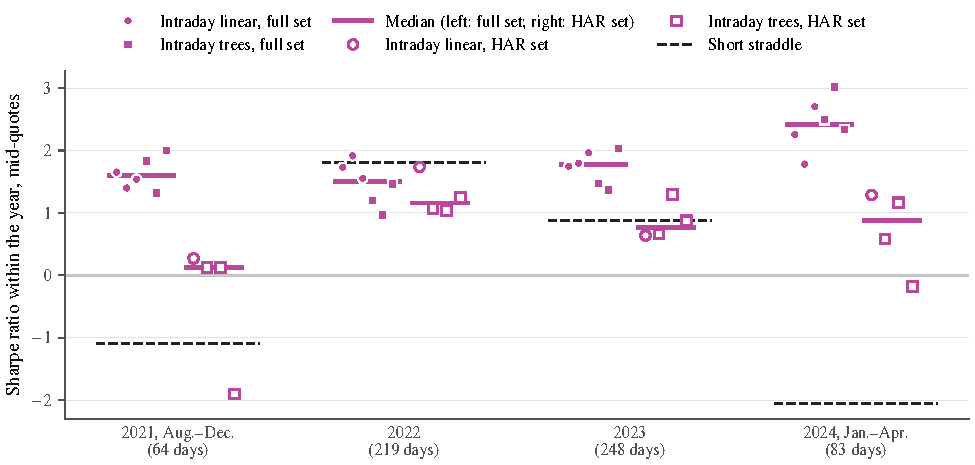
\includegraphics[width=\linewidth]{generated/rehaul_econ_byyear.pdf}
\caption{Sharpe ratio of the sign strategy by calendar year, at mid-quotes, on the \rheSzDays{} post-warmup days of $\mathcal T_{\mathrm{opt}}$. Each point is $\SR_y$, the Sharpe ratio of the year's daily returns annualized by the square root of that year's option days per calendar year (Section~\ref{sec:rh_econ_measures}); the paper's $\SR$ pools the days of all years. Within each year, the left group shows the six intraday forecasts on the full predictor set (filled) and the right group the \rhemHarDistinctWord{} distinct forecasts on the HAR benchmark set (open; the ridge, lasso and elastic net forecasts coincide, Table~\ref{tab:rh_econ_main}); circles are linear models, squares tree ensembles, and the short magenta lines the group medians (full set: \rhemByYearFullMedOne{}, \rhemByYearFullMedTwo{}, \rhemByYearFullMedThree{}, \rhemByYearFullMedFour{}; HAR set: \rhemByYearHarMedOne{}, \rhemByYearHarMedTwo{}, \rhemByYearHarMedThree{}, \rhemByYearHarMedFour{}). The long dashed line marks the short straddle (\rhemByYearShortOne{}, \rhemByYearShortTwo{}, \rhemByYearShortThree{}, \rhemByYearShortFour{}). The years hold \rhemNyOne{}, \rhemNyTwo{}, \rhemNyThree{}, \rhemNyFour{} option days, and the first and last are partial.}
\label{fig:rh_econ_byyear}
\end{figure}
